% -*- root: ../../../thesis.tex -*-





%% -------------------------------------------------------------------------
\section{Data Cleaning}
Before combining into a common database, more than 30 datasets have been cleaned and homogenised separately.
Cleaning steps comprised the following steps (Figure~\ref{fig:data_cleaning} gives a graphical overview):

\begin{enumerate}
	\item Structure: Datasets have been adjusted to the database structure.
	\item Coordinates: Coordinates have been transformed to a common Coordinate Reference System (DHDN / 3-Grad Gauss-Krüger Zone 3 (EPSG:31467)) and duplicates merged.
	\item Chemicals: Chemical names and identifiers have been unified using the webchem package (https://github.com/ropensci/webchem).
	\item  Identifiers: Unique identifiers have been assigned.
	\item Units: All concentrations have been converted to $\mu g/L$. Values below limit of quantification were set to zero (and can be used to identify non-detects).
	\item Other meta-data: meta-data has been standardised.
	\item Temporal resolution: The temporal resolution of the database is 1 day. Samplings below this resolution have been aggregated by the maximum daily value.
	\item Validity Checks: Simple rules for validity checks have been implemented.
\end{enumerate}

\begin{figure}[ht]
	\centering
	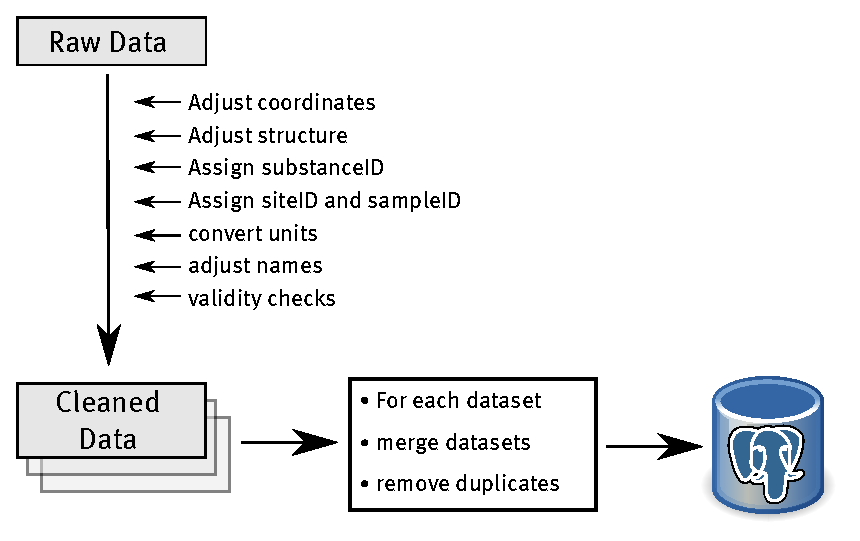
\includegraphics[width = \textwidth]{appendix/smallstreams/one/data_cleaning}
	\caption[Overview on data cleaning steps.]{Overview on data cleaning steps. After cleaning, data have been stored in a relational spatial PostgreSQL database.}
	\label{fig:data_cleaning}
\end{figure}



%% -------------------------------------------------------------------------
\FloatBarrier

\clearpage
\section{Overview on compiled data}
% Overview samples
% table generated in do_overview.R
\begin{sidewaystable}[H]
\centering
\caption[Overview on chemical samples.]{Overview on chemical samples. Only data from running waters and grab
sampling is shown. \textsuperscript{a}: Abbreviations according to ISO 3166-2:DE. 
      \textsuperscript{b}: Including metabolites}\label{tab:phch_overview}
\begin{tabular}{p{2.7cm}lllR{2cm}R{2cm}R{2cm}}
  \toprule
name & abbrv.\textsuperscript{a} & Begin & End & No. sites & No.samples & No. pesticides\textsuperscript{b} \\ 
  \midrule
Baden-Württemberg & BW & 2005-03-10 & 2014-10-02 & 7 & 172 & 98 \\ 
  Bavaria & BY & 2006-04-19 & 2013-12-17 & 13 & 218 & 155 \\ 
  Hesse & HE & 2007-01-15 & 2014-12-18 & 65 & 2411 & 144 \\ 
  Mecklenburg-Western Pomerania & MV & 2005-03-08 & 2014-12-17 & 130 & 1503 & 227 \\ 
  Lower Saxony & NI & 2014-03-24 & 2014-10-13 & 1 & 7 & 226 \\ 
  North Rhine-Westphalia & NW & 2005-01-18 & 2015-01-22 & 1139 & 8536 & 198 \\ 
  Rhineland-Palatinate & RP & 2008-01-02 & 2013-12-18 & 7 & 341 & 236 \\ 
  Schleswig-Holstein & SH & 2005-04-26 & 2014-11-26 & 269 & 1380 & 180 \\ 
  Saarland & SL & 2005-01-03 & 2013-11-25 & 2 & 104 & 57 \\ 
  Saxony & SN & 2005-01-02 & 2013-12-18 & 606 & 9141 & 173 \\ 
  Saxony-Anhalt & ST & 2005-01-24 & 2015-03-19 & 30 & 416 & 88 \\ 
  Thuringia & TH & 2005-06-16 & 2014-12-08 & 32 & 514 & 63 \\ 
   \midrule
 & Total & 2005-01-02 & 2015-03-19 & 2301 & 24743 & 478 \\ 
   \bottomrule
\end{tabular}
\end{sidewaystable}



\clearpage


\begin{landscape}
\begin{figure}[h]
	\centering
	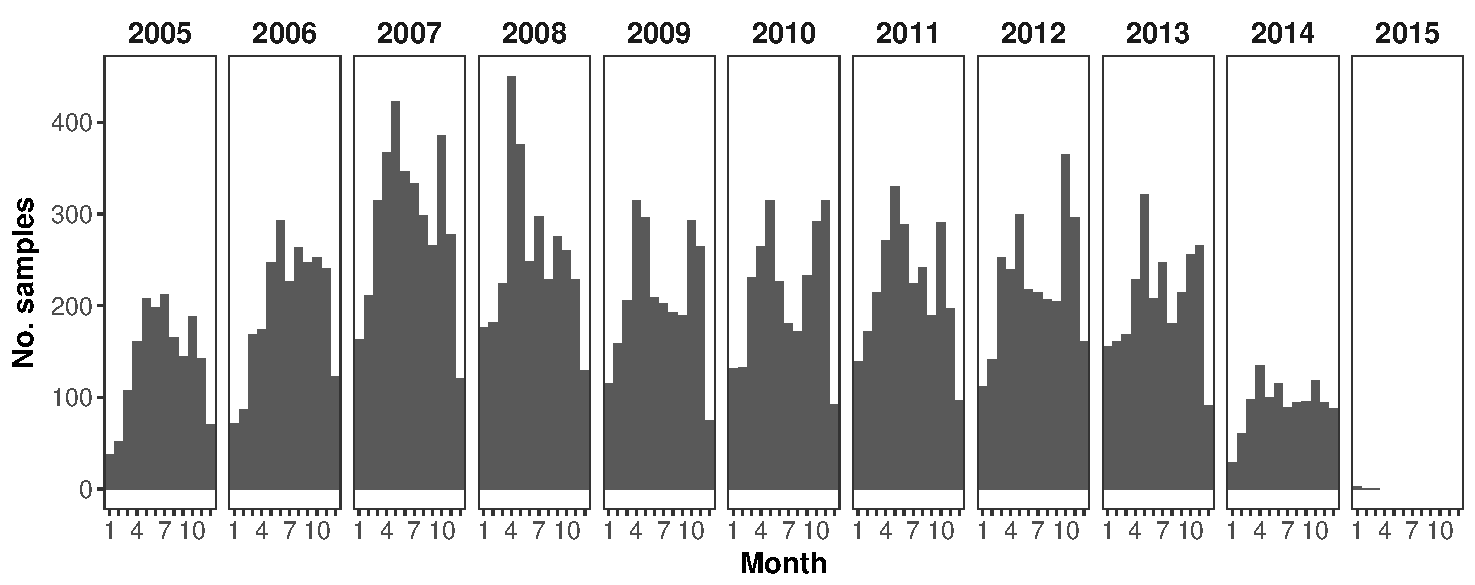
\includegraphics[width = \textheight]{appendix/smallstreams/one/temporal}
	\caption{Number of sampling occasions per year and month.}
	\label{fig:temporal}
\end{figure}
\end{landscape}

\clearpage


\begin{figure}[h]
	\centering
	\vspace{-1.5cm}
	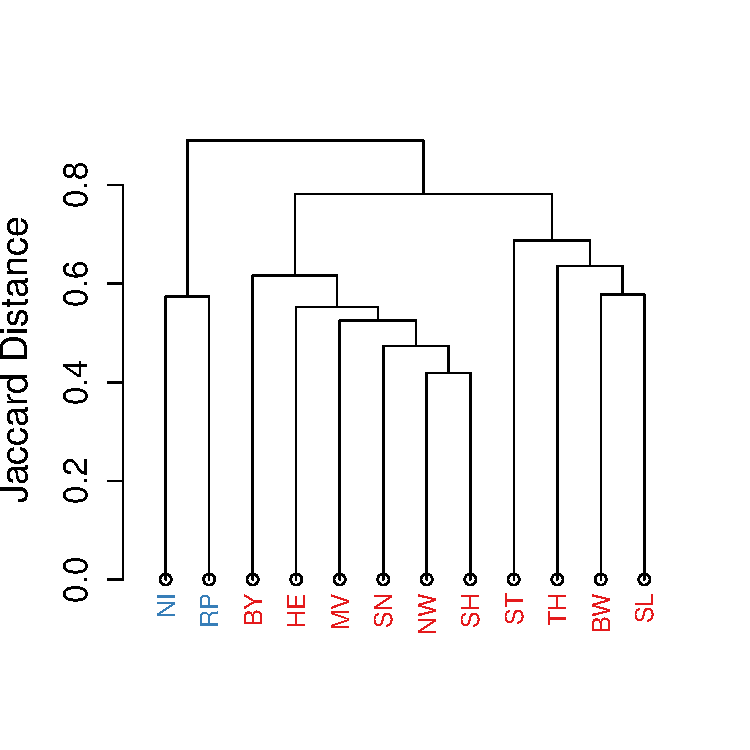
\includegraphics[width = 0.6\textwidth]{appendix/smallstreams/one/varclus}
	\vspace{-1cm}
	\caption[Complete Linkage Cluster Dendrogram of Jaccard Similarity of analysed compound spectra between federal states.]{Complete Linkage Cluster Dendrogram of Jaccard Similarity of analysed compound spectra between federal states. Abbreviations of state names according to ISO 3166-2:DE.}
	\label{fig:varclus}
\end{figure}



\begin{figure}[h]
	\centering
	\vspace{-1.5cm} 
	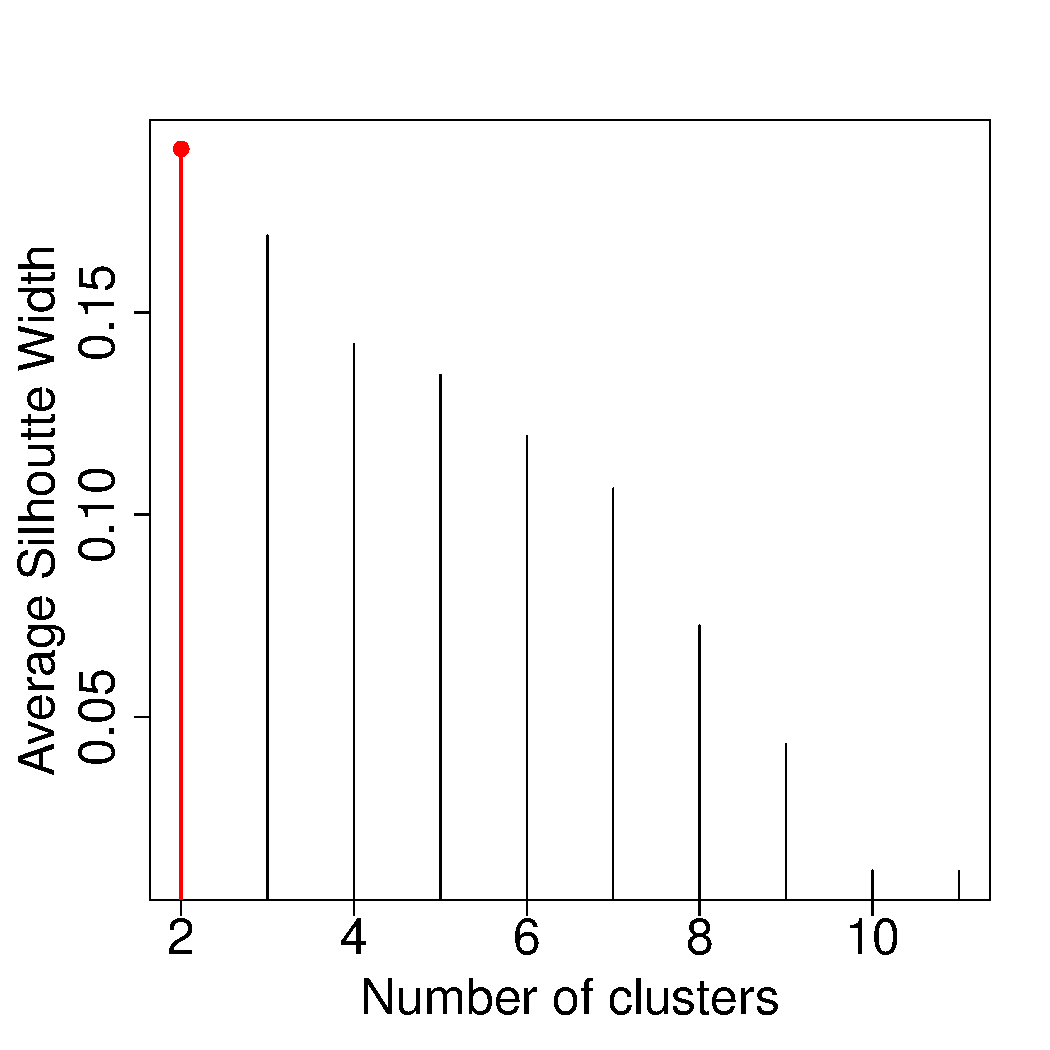
\includegraphics[width = 0.5\textwidth]{appendix/smallstreams/one/silhouette}
	\caption[Average silhouette width for different cluster sizes.]{Average silhouette width for different cluster sizes of complete linkage clustering of jaccard similarity of analysed compound spectra between federal states. Two clusters showed the maximum silhouette width.}
	\label{fig:silhouette}
\end{figure}

% Overview variables
% table generated in do_overview.R
\clearpage
\footnotesize
% -*- root: ../../../thesis.tex -*-

\begin{longtable}{lp{3cm}rlp{1cm}p{1cm}p{1.5cm}}
\caption[Overview on pesticides in the database.]{Overview on pesticides (and metabolites) in the database. \
                    \textsuperscript{a} Authorized in Germany (Source: German Federal Office of Consumer Protection and Food Safety (BVL) as at March 2015). 
                    \textsuperscript{b} Authorized in the European union (Source: EU Pesticides database as at March 2015).
                    \textsuperscript{c} Regulatory Acceptable Concentration [$\mu g/L$] (Source: German Environment Agency (UBA) as at November 2015).} \\ 
  \toprule
 & Name & CAS & Group & Auth. GER\textsuperscript{a} & Auth. EU\textsuperscript{b} & RAC \textsuperscript{c} \\ 
  \midrule
  \endfirsthead
  %
\caption*{\raggedright Table \thetable\ Continued. }\\
        \toprule
 & Name & CAS & Group & Auth. GER\textsuperscript{a} & Auth. EU\textsuperscript{b} & RAC \textsuperscript{c} \\ 
\midrule
\endhead
%
1 & (E)7-(Z)9-Dodecadienylacetat & 55774-32-8 & other & x & x &  \\ 
  2 & (Z)-9-Dodecenylacetat & 16974-11-1 & other & x & x &  \\ 
  3 & 1,3-cis-Dichlorpropen & 10061-01-5 & other &  &  &  \\ 
  4 & 1,3-trans-Dichlorpropen & 10061-02-6 & other &  &  &  \\ 
  5 & 1-(3,4-Dichlorphenyl)urea & 2327-02-8 & metabolite &  &  &  \\ 
  6 & 1-(4-Isopropylphenyl)urea & 56046-17-4 & metabolite &  &  &  \\ 
  7 & 1-Decanol & 112-30-1 & other & x & x &  \\ 
  8 & 1-Methylcyclopropen & 3100-04-7 & other & x & x &  \\ 
  9 & 2,4,5-T & 93-76-5 & herbicide &  &  &  \\ 
  10 & 2,4,6-Trichlorphenol & 88-06-2 & metabolite &  &  &  \\ 
  11 & 2,4-D & 94-75-7 & herbicide & x & x & 1.10000 \\ 
  12 & 2,4-DB & 94-82-6 & herbicide &  & x &  \\ 
  13 & 2,4-Dichlorphenol & 120-83-2 & metabolite &  &  &  \\ 
  14 & 2,6-Dichlorobenzamid & 2008-58-4 & metabolite &  &  &  \\ 
  15 & 2-Hydroxydesethylatrazin & 19988-24-0 & metabolite &  &  &  \\ 
  16 & 3-Hydroxy Carbofuran & 16655-82-6 & metabolite &  &  &  \\ 
  17 & 4,6-Dinitro-o-Cresol & 534-52-1 & insecticide &  &  &  \\ 
  18 & 4-tert. Cyclobutylhexanon & 98-53-3 & metabolite &  &  &  \\ 
  19 & AMPA & 1066-51-9 & metabolite &  &  &  \\ 
  20 & Acequinocyl & 57960-19-7 & insecticide & x & x & 9.00000 \\ 
  21 & Acetamiprid & 135410-20-7 & insecticide & x & x & 0.24000 \\ 
  22 & Acetochlor & 34256-82-1 & herbicide &  &  &  \\ 
  23 & Acetochlorsulfonsäure & 187022-11-3 & metabolite &  &  &  \\ 
  24 & Acetochlorsäure & 194992-44-4 & metabolite &  &  &  \\ 
  25 & Acifluorfen & 50594-66-6 & herbicide &  &  &  \\ 
  26 & Aclonifen & 74070-46-5 & herbicide & x & x & 1.06000 \\ 
  27 & Acrinathrin & 101007-06-1 & insecticide &  & x &  \\ 
  28 & Alachlor & 15972-60-8 & herbicide &  &  &  \\ 
  29 & Aldicarb & 116-06-3 & insecticide &  &  &  \\ 
  30 & Aldrin & 309-00-2 & insecticide &  &  &  \\ 
  31 & Ametoctradin & 865318-97-4 & fungicide & x & x &  \\ 
  32 & Ametryn & 834-12-8 & herbicide &  &  &  \\ 
  33 & Amidosulfuron & 120923-37-7 & herbicide & x & x &  \\ 
  34 & Aminopyralid & 150114-71-9 & herbicide & x & x &  \\ 
  35 & Amisulbrom & 348635-87-0 & fungicide & x & x &  \\ 
  36 & Anthranilsäure\-isopropylamid & 30391-89-0 & metabolite &  &  &  \\ 
  37 & Atraton & 1610-17-9 & herbicide &  &  &  \\ 
  38 & Atrazin & 1912-24-9 & herbicide &  &  &  \\ 
  39 & Atrazin, 2-Hydroxy & 2163-68-0 & metabolite &  &  &  \\ 
  40 & Avermectin B1a & 71751-41-2 & insecticide & x & x &  \\ 
  41 & Azadirachtin (Neem) & 11141-17-6 & insecticide & x & x &  \\ 
  42 & Azinphos-ethyl & 2642-71-9 & insecticide &  &  &  \\ 
  43 & Azinphos-methyl & 86-50-0 & insecticide &  &  &  \\ 
  44 & Aziprotryn & 4658-28-0 & herbicide &  &  &  \\ 
  45 & Azoxystrobin & 131860-33-8 & fungicide & x & x & 0.55000 \\ 
  46 & Azoxystrobin-CA &  & metabolite &  &  &  \\ 
  47 & Beflubutamid & 113614-08-7 & herbicide & x & x &  \\ 
  48 & Benalaxyl & 71626-11-4 & fungicide & x & x & 20.00000 \\ 
  49 & Benazolin & 3813-05-6 & herbicide &  &  &  \\ 
  50 & Bensulfuron-methyl & 83055-99-6 & herbicide &  & x &  \\ 
  51 & Bentazon & 25057-89-0 & herbicide & x & x & 535.00000 \\ 
  52 & Benthiavalicarb & 413615-35-7 & fungicide & x & x &  \\ 
  53 & Benzoesäure & 65-85-0 & fungicide & x & x &  \\ 
  54 & Betacypermethrin & 65731-84-2 & insecticide &  & x &  \\ 
  55 & Bifenazate & 149877-41-8 & insecticide & x & x &  \\ 
  56 & Bifenox & 42576-02-3 & herbicide & x & x &  \\ 
  57 & Bifenthrin & 82657-04-3 & insecticide &  & x & 0.00050 \\ 
  58 & Bixafen & 581809-46-3 & fungicide & x & x & 0.46000 \\ 
  59 & Boscalid & 188425-85-6 & fungicide & x & x & 12.50000 \\ 
  60 & Bromacil & 314-40-9 & herbicide &  &  &  \\ 
  61 & Bromadiolon & 28772-56-7 & other &  & x &  \\ 
  62 & Bromocyclen & 1715-40-8 & insecticide &  &  &  \\ 
  63 & Bromoxynil & 1689-84-5 & herbicide & x & x & 3.30000 \\ 
  64 & Bupirimat & 41483-43-6 & fungicide &  & x &  \\ 
  65 & Buturon & 3766-60-7 & herbicide &  &  &  \\ 
  66 & Captan & 133-06-2 & fungicide & x & x & 5.00000 \\ 
  67 & Carbendazim & 10605-21-7 & fungicide &  &  & 0.15000 \\ 
  68 & Carbetamid & 16118-49-3 & herbicide &  & x &  \\ 
  69 & Carbofuran & 1563-66-2 & insecticide &  &  &  \\ 
  70 & Carboxin & 5234-68-4 & fungicide &  & x &  \\ 
  71 & Carfentrazone-ethyl & 128639-02-1 & herbicide & x & x & 0.31000 \\ 
  72 & Chloramben & 133-90-4 & herbicide &  &  &  \\ 
  73 & Chlorantraniliprole & 500008-45-7 & insecticide & x & x & 0.35500 \\ 
  74 & Chlorbromuron & 13360-45-7 & herbicide &  &  &  \\ 
  75 & Chlordan & 57-74-9 & insecticide &  &  &  \\ 
  76 & Chlorfenac & 85-34-7 & herbicide &  &  &  \\ 
  77 & Chlorfenvinphos & 470-90-6 & insecticide &  &  &  \\ 
  78 & Chlorfluazuron & 71422-67-8 & insecticide &  &  &  \\ 
  79 & Chloridazon & 1698-60-8 & herbicide & x & x & 56.00000 \\ 
  80 & Chlormequat & 7003-89-6 & other & x & x &  \\ 
  81 & Chloroxuron & 1982-47-4 & herbicide &  &  &  \\ 
  82 & Chlorpropham & 101-21-3 & herbicide & x & x &  \\ 
  83 & Chlorpyrifos & 2921-88-2 & insecticide &  & x & 0.00050 \\ 
  84 & Chlorpyriphos methyl & 5598-13-0 & insecticide &  & x &  \\ 
  85 & Chlorsulfuron & 64902-72-3 & herbicide &  &  &  \\ 
  86 & Chlorthalonil & 1897-45-6 & fungicide & x & x &  \\ 
  87 & Chlorthalonil-SA &  & metabolite &  &  &  \\ 
  88 & Chlortoluron & 15545-48-9 & herbicide & x & x & 2.30000 \\ 
  89 & Cinidon-ethyl & 142891-20-1 & herbicide &  &  &  \\ 
  90 & Clethodim & 99129-21-2 & herbicide & x & x &  \\ 
  91 & Clodinafop & 114420-56-3 & herbicide & x & x &  \\ 
  92 & Clodinafop-propargyl & 105512-06-9 & herbicide &  &  &  \\ 
  93 & Clofentezin & 74115-24-5 & insecticide &  & x &  \\ 
  94 & Clomazon & 81777-89-1 & herbicide & x & x & 5.70000 \\ 
  95 & Clopyralid & 1702-17-6 & herbicide & x & x & 1080.00000 \\ 
  96 & Cloquintocet-mexyl & 99607-70-2 & other &  & x &  \\ 
  97 & Clothianidin & 210880-92-5 & insecticide & x & x & 0.00700 \\ 
  98 & Codlemone (Codlelure) & 33956-49-9 & other & x & x &  \\ 
  99 & Coumaphos & 56-72-4 & insecticide &  &  &  \\ 
  100 & Crimidin & 535-89-7 & other &  &  &  \\ 
  101 & Cyanazin & 21725-46-2 & herbicide &  &  &  \\ 
  102 & Cyazofamid & 120116-88-3 & fungicide & x & x &  \\ 
  103 & Cyclanilide & 113136-77-9 & other &  &  &  \\ 
  104 & Cycloat & 1134-23-2 & herbicide &  &  &  \\ 
  105 & Cycloxidim & 101205-02-1 & herbicide & x & x &  \\ 
  106 & Cyflufenamid & 180409-60-3 & fungicide & x & x &  \\ 
  107 & Cyfluthrin (Summe Isomere) & 68359-37-5 & insecticide &  &  &  \\ 
  108 & Cyhalothrin (Summe Isomere) & 91465-08-6 & insecticide & x & x &  \\ 
  109 & Cymoxanil & 57966-95-7 & fungicide & x & x & 4.40000 \\ 
  110 & Cypermetryn & 52315-07-8 & insecticide & x & x & 0.00100 \\ 
  111 & Cyproconazol & 94361-06-5 & fungicide & x & x &  \\ 
  112 & Cyprodinil & 121552-61-2 & fungicide & x & x & 0.75000 \\ 
  113 & Cyromazin & 66215-27-8 & insecticide &  & x &  \\ 
  114 & Daminozid & 1596-84-5 & other & x & x &  \\ 
  115 & Deiquat & 2764-72-9 & herbicide & x & x &  \\ 
  116 & Deltamethrin & 52918-63-5 & insecticide & x & x &  \\ 
  117 & Demeton-O & 298-03-3 & insecticide &  &  &  \\ 
  118 & Demeton-S & 126-75-0 & insecticide &  &  &  \\ 
  119 & Demeton-S-methyl & 919-86-8 & insecticide &  &  &  \\ 
  120 & Demeton-S-methylsulfon & 17040-19-6 & insecticide &  &  &  \\ 
  121 & Desaminometribuzin & 35045-02-4 & metabolite &  &  &  \\ 
  122 & Desethyl-2-hydroxyterbuthylazin & 66753-06-8 & metabolite &  &  &  \\ 
  123 & Desethylatrazin & 6190-65-4 & metabolite &  &  &  \\ 
  124 & Desethylsebuthylazin & 37019-18-4 & metabolite &  &  &  \\ 
  125 & Desethylsimazin & 6190-65-4 & metabolite &  &  &  \\ 
  126 & Desethylterbuthylazin & 30125-63-4 & metabolite &  &  &  \\ 
  127 & Desisopropylatrazin & 1007-28-9 & metabolite &  &  &  \\ 
  128 & Desmedipham & 13684-56-5 & herbicide & x & x &  \\ 
  129 & Desmethyldiuron & 3567-62-2 & metabolite &  &  &  \\ 
  130 & Desmethylisoproturon & 34123-57-4 & metabolite &  &  &  \\ 
  131 & Desmetryn & 1014-69-3 & herbicide &  &  &  \\ 
  132 & Desphenyl-Chloridazon & 6339-19-1 & metabolite &  &  &  \\ 
  133 & Diazinon & 333-41-5 & insecticide &  &  &  \\ 
  134 & Dicamba & 1918-00-9 & herbicide & x & x & 180.00000 \\ 
  135 & Dichlobenil & 1194-65-6 & herbicide &  &  &  \\ 
  136 & Dichlofluanid & 1085-98-9 & fungicide &  &  &  \\ 
  137 & Dichlorprop & 120-36-5 & herbicide &  &  &  \\ 
  138 & Dichlorprop-P & 15165-67-0 & herbicide & x & x &  \\ 
  139 & Dichlorvos & 62-73-7 & insecticide &  &  &  \\ 
  140 & Diclofop & 40843-25-2 & herbicide &  & x &  \\ 
  141 & Dicofol & 115-32-2 & insecticide &  &  &  \\ 
  142 & Dieldrin & 60-57-1 & insecticide &  &  &  \\ 
  143 & Difenacoum & 56073-07-5 & other &  & x &  \\ 
  144 & Difenoconazol & 119446-68-3 & fungicide & x & x & 0.36000 \\ 
  145 & Diflubenzuron & 35367-38-5 & insecticide &  & x &  \\ 
  146 & Diflufenican & 83164-33-4 & herbicide & x & x & 0.02500 \\ 
  147 & Dimefuron & 34205-21-5 & herbicide &  &  & 0.83000 \\ 
  148 & Dimethachlor & 50563-36-5 & herbicide & x & x & 3.50000 \\ 
  149 & Dimethachlor-CA &  & metabolite &  &  &  \\ 
  150 & Dimethachlor\-sulfonsäure &  & metabolite &  &  &  \\ 
  151 & Dimethachlorsäure &  & metabolite &  &  &  \\ 
  152 & Dimethenamid & 87674-68-8 & herbicide &  &  &  \\ 
  153 & Dimethenamid-CA &  & metabolite &  &  &  \\ 
  154 & Dimethenamid-P & 163515-14-8 & herbicide & x & x & 1.35000 \\ 
  155 & Dimethenamid-SA &  & metabolite &  &  &  \\ 
  156 & Dimethenamid\-sulfonsäure &  & metabolite &  &  &  \\ 
  157 & Dimethoat & 60-51-5 & insecticide & x & x & 4.00000 \\ 
  158 & Dimethomorph & 110488-70-5 & fungicide & x & x & 5.60000 \\ 
  159 & Dimoxystrobin & 149961-52-4 & fungicide & x & x & 0.03160 \\ 
  160 & Diniconazol & 83657-24-3 & fungicide &  &  &  \\ 
  161 & Dinoseb & 88-85-7 & herbicide &  &  &  \\ 
  162 & Dinotefuran & 165252-70-0 & insecticide &  &  &  \\ 
  163 & Dinoterb & 1420-07-1 & herbicide &  &  &  \\ 
  164 & Disulfoton & 298-04-4 & insecticide &  &  &  \\ 
  165 & Dithianon & 3347-22-6 & fungicide & x & x & 0.78000 \\ 
  166 & Diuron & 330-54-1 & herbicide &  & x & 0.79000 \\ 
  167 & Dodin & 2439-10-3 & fungicide & x & x & 5.33000 \\ 
  168 & Endosulfan, alpha & 959-98-8 & insecticide &  &  &  \\ 
  169 & Endosulfan, beta & 33213-65-9 & insecticide &  &  &  \\ 
  170 & Endosulfansulfat & 1031-07-8 & metabolite &  &  &  \\ 
  171 & Endrin & 72-20-8 & insecticide &  &  &  \\ 
  172 & Epoxiconazol & 133855-98-8 & fungicide & x & x & 0.53750 \\ 
  173 & Esfenvalerat & 66230-04-4 & insecticide & x & x &  \\ 
  174 & Etaconazol & 60207-93-4 & fungicide &  &  &  \\ 
  175 & Ethidimuron & 30043-49-3 & herbicide &  &  &  \\ 
  176 & Ethirimol & 23947-60-6 & fungicide &  &  &  \\ 
  177 & Ethofenprox & 80844-07-1 & insecticide & x & x &  \\ 
  178 & Ethofumesat & 26225-79-6 & herbicide & x & x & 24.00000 \\ 
  179 & Etrimfos & 38260-54-7 & insecticide &  &  &  \\ 
  180 & Famoxadone & 131807-57-3 & fungicide & x & x &  \\ 
  181 & Fenamidon & 161326-34-7 & fungicide & x & x &  \\ 
  182 & Fenamiphos & 22224-92-6 & insecticide &  & x &  \\ 
  183 & Fenarimol & 60168-88-9 & fungicide &  &  &  \\ 
  184 & Fenazaquin & 120928-09-8 & insecticide & x & x &  \\ 
  185 & Fenhexamid & 126833-17-8 & fungicide & x & x & 10.10000 \\ 
  186 & Fenitrothion & 122-14-5 & insecticide &  &  &  \\ 
  187 & Fenoprop & 93-72-1 & herbicide &  &  &  \\ 
  188 & Fenoxaprop & 95617-09-7 & herbicide &  &  &  \\ 
  189 & Fenoxaprop-p & 113158-40-0 & herbicide & x & x &  \\ 
  190 & Fenoxaprop-p-ethyl & 71283-80-2 & herbicide &  &  &  \\ 
  191 & Fenoxycarb & 72490-01-8 & insecticide &  & x &  \\ 
  192 & Fenpropidin & 67306-00-7 & fungicide & x & x &  \\ 
  193 & Fenpropimorph & 67564-91-4 & fungicide & x & x & 0.19500 \\ 
  194 & Fenpyroximat & 134098-61-6 & insecticide & x & x &  \\ 
  195 & Fenthion & 55-38-9 & insecticide &  &  &  \\ 
  196 & Fenuron & 101-42-8 & herbicide &  &  &  \\ 
  197 & Fipronil & 120068-37-3 & insecticide &  & x & 0.00077 \\ 
  198 & Flamprop & 58667-63-3 & herbicide &  &  &  \\ 
  199 & Flazasulfuron & 104040-78-0 & herbicide & x & x &  \\ 
  200 & Flonicamid & 158062-67-0 & insecticide & x & x & 310.00000 \\ 
  201 & Florasulam & 145701-23-1 & herbicide & x & x &  \\ 
  202 & Fluazifop & 69335-91-7 & herbicide &  &  & 146.00000 \\ 
  203 & Fluazifop-P & 83066-88-0 & herbicide & x & x & 146.00000 \\ 
  204 & Fluazifop-P-butyl & 79241-46-6 & herbicide &  &  & 7.70000 \\ 
  205 & Fluazifop-butyl & 69806-50-4 & herbicide &  &  & 7.70000 \\ 
  206 & Fluazinam & 79622-59-6 & fungicide & x & x & 0.26000 \\ 
  207 & Fluchloralin & 33245-39-5 & herbicide &  &  &  \\ 
  208 & Fludioxonil & 131341-86-1 & fungicide & x & x & 0.50000 \\ 
  209 & Flufenacet & 142459-58-3 & herbicide & x & x & 2.40000 \\ 
  210 & Flufenacet-SA &  & metabolite &  &  &  \\ 
  211 & Flufenoxuron & 101463-69-8 & insecticide &  &  &  \\ 
  212 & Flumioxazin & 103361-09-7 & herbicide & x & x &  \\ 
  213 & Fluometuron & 2164-17-2 & herbicide &  & x &  \\ 
  214 & Fluopicolide & 239110-15-7 & fungicide & x & x &  \\ 
  215 & Fluopyram & 658066-35-4 & fungicide & x & x & 5.12000 \\ 
  216 & Fluoxastrobin & 361377-29-9 & fungicide & x & x &  \\ 
  217 & Flupyrsulfuron & 150315-10-9 & herbicide & x & x &  \\ 
  218 & Fluquinconazole & 136426-54-5 & fungicide & x & x & 0.80000 \\ 
  219 & Flurochloridon & 61213-25-0 & herbicide &  & x &  \\ 
  220 & Fluroxypyr & 69377-81-7 & herbicide & x & x & 16.00000 \\ 
  221 & Fluroxypyr-methylheptyl & 81406-37-3 & herbicide &  &  &  \\ 
  222 & Flurtamone & 96525-23-4 & herbicide & x & x & 0.99000 \\ 
  223 & Flusilazol & 85509-19-9 & fungicide &  &  & 1.10000 \\ 
  224 & Flutolanil & 66332-96-5 & fungicide & x & x &  \\ 
  225 & Flutriafol & 76674-21-0 & fungicide &  & x &  \\ 
  226 & Fluxapyroxad & 907204-31-3 & fungicide & x & x &  \\ 
  227 & Folpet & 133-07-3 & fungicide & x & x &  \\ 
  228 & Foramsulfuron & 173159-57-4 & herbicide & x & x & 0.09500 \\ 
  229 & Fosetyl & 15845-66-6 & fungicide & x & x &  \\ 
  230 & Fosthiazat & 98886-44-3 & other & x & x &  \\ 
  231 & Fuberidazol & 3878-19-1 & fungicide & x & x &  \\ 
  232 & Furalaxyl & 57646-30-7 & fungicide &  &  &  \\ 
  233 & Furmecyclox & 60568-05-0 & fungicide &  &  &  \\ 
  234 & Glufosinat & 51276-47-2 & herbicide & x & x &  \\ 
  235 & Glyphosate & 1071-83-6 & herbicide & x & x & 100.00000 \\ 
  236 & HCH, gamma (Lindan) & 58-89-9 & insecticide &  &  &  \\ 
  237 & Haloxyfop & 69806-34-4 & herbicide &  &  &  \\ 
  238 & Haloxyfop-P & 95977-29-0 & herbicide & x & x &  \\ 
  239 & Haloxyfop-ethoxyethyl & 87237-48-7 & herbicide &  &  &  \\ 
  240 & Heptachlor & 76-44-8 & insecticide &  &  &  \\ 
  241 & Heptachlorepoxid & 1024-57-3 & metabolite &  &  &  \\ 
  242 & Heptenophos & 23560-59-0 & insecticide &  &  &  \\ 
  243 & Hexachlorbenzen & 118-74-1 & fungicide &  &  &  \\ 
  244 & Hexachlorophen & 70-30-4 & other &  &  &  \\ 
  245 & Hexaconazol & 79983-71-4 & fungicide &  &  &  \\ 
  246 & Hexaflumuron & 86479-06-3 & insecticide &  &  &  \\ 
  247 & Hexazinon & 51235-04-2 & herbicide &  &  &  \\ 
  248 & Hexythiazox & 78587-05-0 & insecticide & x & x &  \\ 
  249 & Hymexazol & 10004-44-1 & fungicide & x & x &  \\ 
  250 & Icaridinsäure &  & metabolite &  &  &  \\ 
  251 & Imazalil & 35554-44-0 & fungicide & x & x &  \\ 
  252 & Imazamox & 114311-32-9 & herbicide & x & x &  \\ 
  253 & Imazapic & 104098-48-8 & herbicide &  &  &  \\ 
  254 & Imazaquin & 81335-37-7 & herbicide &  & x &  \\ 
  255 & Imazethapyr & 81335-77-5 & herbicide &  &  &  \\ 
  256 & Imazosulfuron & 122548-33-8 & herbicide & x & x &  \\ 
  257 & Imidacloprid & 138261-41-3 & insecticide & x & x & 0.00900 \\ 
  258 & Indoxacarb & 173584-44-6 & insecticide & x & x &  \\ 
  259 & Iodosulfuron & 185119-76-0 & herbicide & x & x & 0.07900 \\ 
  260 & Iodosulfuron-methyl & 144550-06-1 & herbicide &  &  &  \\ 
  261 & Iodosulfuron-methyl-sodium & 144550-36-7 & herbicide &  &  &  \\ 
  262 & Ioxynil & 1689-83-4 & herbicide & x &  & 2.70000 \\ 
  263 & Iprodion & 36734-19-7 & fungicide & x & x &  \\ 
  264 & Iprovalicarb & 140923-17-7 & fungicide & x & x & 189.00000 \\ 
  265 & Isodrin & 465-73-6 & insecticide &  &  &  \\ 
  266 & Isophenphos & 25311-71-1 & insecticide &  &  &  \\ 
  267 & Isoproturon & 34123-59-6 & herbicide & x & x & 1.30000 \\ 
  268 & Isopyrazam & 881685-58-1 & fungicide & x & x &  \\ 
  269 & Isoxaben & 82558-50-7 & herbicide & x & x &  \\ 
  270 & Isoxaflutole & 141112-29-0 & herbicide & x & x &  \\ 
  271 & Karbutylat & 4849-32-5 & herbicide &  &  &  \\ 
  272 & Kresoxim-methyl & 143390-89-0 & fungicide & x & x & 1.00000 \\ 
  273 & Kresoximsäure &  & metabolite &  &  &  \\ 
  274 & Lenacil & 2164-08-1 & herbicide & x & x & 0.65000 \\ 
  275 & Linuron & 330-55-2 & herbicide &  & x &  \\ 
  276 & MCPA & 94-74-6 & herbicide & x & x & 9.00000 \\ 
  277 & MCPB & 94-81-5 & herbicide &  & x &  \\ 
  278 & Malathion & 121-75-5 & insecticide &  & x &  \\ 
  279 & Mancozeb & 8018-01-7 & fungicide & x & x & 0.21900 \\ 
  280 & Mandipropamid & 374726-62-2 & fungicide & x & x & 7.60000 \\ 
  281 & Maneb & 12427-38-2 & fungicide & x & x &  \\ 
  282 & Mecoprop & 93-65-2 & herbicide &  & x & 160.00000 \\ 
  283 & Mefenpyr-diethyl & 135591-00-3 & other & x &  &  \\ 
  284 & Mepanipyrim & 110235-47-7 & fungicide & x & x &  \\ 
  285 & Mepiquat & 15302-91-7 & other & x & x &  \\ 
  286 & Mepronil & 55814-41-0 & fungicide &  &  &  \\ 
  287 & Meptyldinocap & 131-72-6 & fungicide &  & x &  \\ 
  288 & Mesosulfuron & 400852-66-6 & herbicide & x & x &  \\ 
  289 & Mesotrion & 104206-82-8 & herbicide & x & x &  \\ 
  290 & Metaflumizone & 139968-49-3 & insecticide & x & x &  \\ 
  291 & Metalaxyl & 57837-19-1 & fungicide &  & x & 46.00000 \\ 
  292 & Metalaxyl-CA & 75596-99-5 & metabolite &  &  &  \\ 
  293 & Metalaxyl-CA2 & 104390-56-9 & metabolite &  &  &  \\ 
  294 & Metalaxyl-M & 70630-17-0 & fungicide & x & x & 46.00000 \\ 
  295 & Metaldehyd & 108-62-3 & other & x & x &  \\ 
  296 & Metamitron & 41394-05-2 & herbicide & x & x & 38.00000 \\ 
  297 & Metamitron-Desamino & 36993-94-9 & metabolite &  &  &  \\ 
  298 & Metazachlor & 67129-08-2 & herbicide & x & x & 0.88000 \\ 
  299 & Metazachlor\-dicarbonsäure &  & metabolite &  &  &  \\ 
  300 & Metazachlor\-sulfonsäure & 172960-62-2 & metabolite &  &  &  \\ 
  301 & Metazachlorsäure & 1231244-60-2 & metabolite &  &  &  \\ 
  302 & Metconazol & 125116-23-6 & fungicide & x & x &  \\ 
  303 & Methabenzthiazuron & 18691-97-9 & herbicide &  &  &  \\ 
  304 & Methamidophos & 10265-92-6 & insecticide &  &  & 2.60000 \\ 
  305 & Methidathion & 950-37-8 & insecticide &  &  &  \\ 
  306 & Methiocarb & 2032-65-7 & insecticide & x & x & 0.01000 \\ 
  307 & Methobromuron & 3060-89-7 & herbicide &  & x & 2.00000 \\ 
  308 & Methomyl & 16752-77-5 & insecticide &  & x &  \\ 
  309 & Methoprotryn & 841-06-5 & herbicide &  &  &  \\ 
  310 & Methoxychlor & 72-43-5 & insecticide &  &  &  \\ 
  311 & Methoxyfenozid & 161050-58-4 & insecticide & x & x &  \\ 
  312 & Methyldesphenyl-Chloridazon & 17254-80-7 & metabolite &  &  &  \\ 
  313 & Metiram & 9006-42-2 & fungicide & x & x &  \\ 
  314 & Metolachlor & 51218-45-2 & herbicide &  &  &  \\ 
  315 & Metolachlor\-sulfonsäure & 171118-09-5 & metabolite &  &  &  \\ 
  316 & Metolachlorsäure & 152019-73-3 & metabolite &  &  &  \\ 
  317 & Metosulam & 139528-85-1 & herbicide & x & x &  \\ 
  318 & Metoxuron & 19937-59-8 & herbicide &  &  &  \\ 
  319 & Metrafenon & 220899-03-6 & fungicide & x & x &  \\ 
  320 & Metribuzin & 21087-64-9 & herbicide & x & x & 0.58400 \\ 
  321 & Metsulfuron & 79510-48-8 & herbicide & x & x &  \\ 
  322 & Metsulfuron-methyl & 74223-64-6 & herbicide &  &  &  \\ 
  323 & Mevinphos & 7786-34-7 & insecticide &  &  &  \\ 
  324 & Milbemectin & 51596-11-3 & insecticide & x & x &  \\ 
  325 & Mirex & 2385-85-5 & insecticide &  &  &  \\ 
  326 & Monolinuron & 1746-81-2 & herbicide &  &  &  \\ 
  327 & Monuron & 150-68-5 & herbicide &  &  &  \\ 
  328 & Myclobutanil & 88671-89-0 & fungicide & x & x & 2.40000 \\ 
  329 & Napropamid & 15299-99-7 & herbicide & x & x & 6.70000 \\ 
  330 & Neburon & 555-37-3 & herbicide &  &  &  \\ 
  331 & Nicosulfuron & 111991-09-4 & herbicide & x & x & 0.08500 \\ 
  332 & Nitenpyram & 120738-89-8 & insecticide &  &  &  \\ 
  333 & Nitrofen & 1836-75-5 & herbicide &  &  &  \\ 
  334 & Norflurazon & 27314-13-2 & herbicide &  &  &  \\ 
  335 & Omethoat & 1113-02-6 & insecticide &  &  &  \\ 
  336 & Orysastrobin & 248593-16-0 & fungicide &  &  &  \\ 
  337 & Oxadiazon & 19666-30-9 & herbicide &  & x &  \\ 
  338 & Oxadixyl & 77732-09-3 & fungicide &  &  &  \\ 
  339 & Oxamyl & 23135-22-0 & insecticide &  & x &  \\ 
  340 & Oxydemeton-methyl & 301-12-2 & insecticide &  &  & 1.10000 \\ 
  341 & Paclobutrazol & 76738-62-0 & other & x & x &  \\ 
  342 & Parathion-ethyl & 56-38-2 & insecticide &  &  &  \\ 
  343 & Parathion-methyl & 298-00-0 & insecticide &  &  &  \\ 
  344 & Pelargonsäure & 112-05-0 & herbicide & x & x &  \\ 
  345 & Penconazol & 66246-88-6 & fungicide & x & x & 3.20000 \\ 
  346 & Pencycuron & 66063-05-6 & fungicide & x & x &  \\ 
  347 & Pendimethalin & 40487-42-1 & herbicide & x & x & 0.63000 \\ 
  348 & Penflufen & 494793-67-8 & fungicide &  & x &  \\ 
  349 & Penoxsulam & 219714-96-2 & herbicide & x & x &  \\ 
  350 & Permethrin & 52645-53-1 & insecticide &  &  &  \\ 
  351 & Pethoxamid & 106700-29-2 & herbicide & x & x & 1.77200 \\ 
  352 & Phenmedipham & 13684-63-4 & herbicide & x & x &  \\ 
  353 & Phoxim & 14816-18-3 & insecticide &  &  & 0.00700 \\ 
  354 & Picloram & 1918-02-1 & herbicide & x & x &  \\ 
  355 & Picolinafen & 137641-05-5 & herbicide & x & x & 0.03600 \\ 
  356 & Picoxystrobin & 117428-22-5 & fungicide & x & x & 0.60000 \\ 
  357 & Pinoxaden & 243973-20-8 & herbicide & x &  &  \\ 
  358 & Pirimicarb & 23103-98-2 & insecticide & x & x & 0.09000 \\ 
  359 & Pirimicarb-desmethyl & 30614-22-3 & metabolite &  &  &  \\ 
  360 & Pirimiphos-ethyl & 23505-41-1 & insecticide &  &  &  \\ 
  361 & Pirimiphos-methyl & 29232-93-7 & insecticide & x & x &  \\ 
  362 & Primisulfuron-methyl & 86209-51-0 & herbicide &  &  &  \\ 
  363 & Prochloraz & 67747-09-5 & fungicide & x & x & 5.00000 \\ 
  364 & Procymidon & 32809-16-8 & fungicide &  &  &  \\ 
  365 & Profoxydim & 139001-49-3 & herbicide &  & x &  \\ 
  366 & Prohexadion & 88805-35-0 & other & x & x &  \\ 
  367 & Prometryn & 7287-19-6 & herbicide &  &  &  \\ 
  368 & Propachlor & 1918-16-7 & herbicide &  &  &  \\ 
  369 & Propamocarb & 24579-73-5 & fungicide & x & x &  \\ 
  370 & Propanil & 709-98-8 & herbicide &  &  &  \\ 
  371 & Propaquizafop & 111479-05-1 & herbicide & x & x &  \\ 
  372 & Propazin & 139-40-2 & herbicide &  &  &  \\ 
  373 & Propetamphos & 31218-83-4 & insecticide &  &  &  \\ 
  374 & Propham & 122-42-9 & herbicide &  &  &  \\ 
  375 & Propiconazol & 60207-90-1 & fungicide & x & x & 2.00000 \\ 
  376 & Propoxur & 114-26-1 & insecticide &  &  &  \\ 
  377 & Propoxycarbazone & 145026-81-9 & herbicide & x & x &  \\ 
  378 & Propyzamid & 23950-58-5 & herbicide & x & x & 34.00000 \\ 
  379 & Proquinazid & 189278-12-4 & fungicide & x & x &  \\ 
  380 & Prosulfocarb & 52888-80-9 & herbicide & x & x & 3.80000 \\ 
  381 & Prosulfuron & 94125-34-5 & herbicide & x & x &  \\ 
  382 & Prothioconazol & 178928-70-6 & fungicide & x & x & 1.71000 \\ 
  383 & Prothioconazol-desthio & 120983-64-4 & metabolite &  &  &  \\ 
  384 & Pymetrozin & 123312-89-0 & insecticide & x & x &  \\ 
  385 & Pyraclostrobin & 175013-18-0 & fungicide & x & x &  \\ 
  386 & Pyraflufen & 129630-17-7 & herbicide & x & x &  \\ 
  387 & Pyrazophos & 13457-18-6 & fungicide &  &  &  \\ 
  388 & Pyrethrum & 8003-34-7 & insecticide & x & x & 0.01400 \\ 
  389 & Pyridaben & 96489-71-3 & insecticide &  & x &  \\ 
  390 & Pyridat & 55512-33-9 & herbicide & x & x &  \\ 
  391 & Pyrifenox & 88283-41-4 & fungicide &  &  &  \\ 
  392 & Pyrimethanil & 53112-28-0 & fungicide & x & x & 8.00000 \\ 
  393 & Pyroxsulam & 422556-08-9 & herbicide & x & x &  \\ 
  394 & Quinalphos & 13593-03-8 & insecticide &  &  &  \\ 
  395 & Quinmerac & 90717-03-6 & herbicide & x & x & 316.00000 \\ 
  396 & Quinoclamin & 2797-51-5 & herbicide & x & x &  \\ 
  397 & Quinoxyfen (5,7-di\-chloro-4-(p-fluoro\-phenoxy)\-quinoline) & 124495-18-7 & fungicide & x & x &  \\ 
  398 & Quintozen & 82-68-8 & fungicide &  &  &  \\ 
  399 & Quizalofop & 76578-12-6 & herbicide &  &  &  \\ 
  400 & Quizalofop-ethyl & 76578-14-8 & herbicide &  &  &  \\ 
  401 & Rimsulfuron & 122931-48-0 & herbicide & x & x & 0.46000 \\ 
  402 & Saflufenacil & 372137-35-4 & herbicide &  &  &  \\ 
  403 & Sebuthylazin & 7286-69-3 & herbicide &  &  &  \\ 
  404 & Secbumeton & 26259-45-0 & herbicide &  &  &  \\ 
  405 & Silthiofam & 175217-20-6 & fungicide & x & x &  \\ 
  406 & Simazin & 122-34-9 & herbicide &  &  &  \\ 
  407 & Simazin, 2-Hydroxy & 2599-11-3 & metabolite &  &  &  \\ 
  408 & Spinosad & 168316-95-8 & insecticide & x & x & 0.06200 \\ 
  409 & Spirodiclofen & 148477-71-8 & insecticide & x & x &  \\ 
  410 & Spiromesifen & 283594-90-1 & insecticide &  & x &  \\ 
  411 & Spiroxamin & 118134-30-8 & fungicide & x & x & 0.13000 \\ 
  412 & Sulcotrion & 99105-77-8 & herbicide & x & x &  \\ 
  413 & Sulfosulfuron & 141776-32-1 & herbicide &  & x &  \\ 
  414 & Sulfurylfluorid & 2699-79-8 & insecticide & x & x &  \\ 
  415 & Tebuconazol & 107534-96-3 & fungicide & x & x & 0.57800 \\ 
  416 & Tebufenozid & 112410-23-8 & insecticide & x & x &  \\ 
  417 & Tebufenpyrad & 119168-77-3 & insecticide & x & x &  \\ 
  418 & Tebutam & 35256-85-0 & herbicide &  &  &  \\ 
  419 & Teflubenzuron & 83121-18-0 & insecticide &  & x &  \\ 
  420 & Tefluthrin & 79538-32-2 & insecticide & x & x &  \\ 
  421 & Telodrin & 297-78-9 & insecticide &  &  &  \\ 
  422 & Tembotrione & 335104-84-2 & herbicide & x & x &  \\ 
  423 & Tepraloxydim & 149979-41-9 & herbicide & x & x &  \\ 
  424 & Terbumeton & 33693-04-8 & herbicide &  &  &  \\ 
  425 & Terbuthylazin & 5915-41-3 & herbicide & x & x & 1.20000 \\ 
  426 & Terbutryn & 886-50-0 & herbicide &  &  &  \\ 
  427 & Terbutylazin-Metabolit CGA 324007 & 309923-18-0 & metabolite &  &  &  \\ 
  428 & Terbutylazin-Metabolit SYN 545666 &  & metabolite &  &  &  \\ 
  429 & Tetraconazol & 112281-77-3 & fungicide & x & x &  \\ 
  430 & Thiabendazol & 148-79-8 & fungicide & x & x &  \\ 
  431 & Thiacloprid & 111988-49-9 & insecticide & x & x & 0.00400 \\ 
  432 & Thiacloprid-SA &  & metabolite &  &  &  \\ 
  433 & Thiamethoxam & 153719-23-4 & insecticide & x & x & 0.04300 \\ 
  434 & Thiencarbazon-methyl & 317815-83-1 & herbicide & x & x &  \\ 
  435 & Thifensulfuron-methyl & 79277-27-3 & herbicide &  &  &  \\ 
  436 & Thifenylsulfuron & 79277-67-1 & herbicide & x & x &  \\ 
  437 & Thiometon & 640-15-3 & insecticide &  &  &  \\ 
  438 & Thiophanat-methyl & 23564-05-8 & fungicide & x & x &  \\ 
  439 & Thiram & 137-26-8 & fungicide & x & x & 0.11000 \\ 
  440 & Tolclofos-methyl & 57018-04-9 & fungicide & x & x &  \\ 
  441 & Tolylfluanid & 731-27-1 & fungicide &  &  &  \\ 
  442 & Topramezone & 210631-68-8 & herbicide & x &  & 0.90000 \\ 
  443 & Tralkoxydim & 87820-88-0 & herbicide &  & x &  \\ 
  444 & Triadimefon & 43121-43-3 & fungicide &  &  &  \\ 
  445 & Triadimenol & 55219-65-3 & fungicide & x & x & 3.40000 \\ 
  446 & Triallat & 2303-17-5 & herbicide &  & x &  \\ 
  447 & Triasulfuron & 82097-50-5 & herbicide & x & x &  \\ 
  448 & Triazophos & 24017-47-8 & insecticide &  &  & 0.03000 \\ 
  449 & Triazoxid & 72459-58-6 & fungicide & x & x &  \\ 
  450 & Tribenuron & 106040-48-6 & herbicide & x & x &  \\ 
  451 & Tribenuron-methyl & 101200-48-0 & herbicide &  &  &  \\ 
  452 & Trichlorfon & 52-68-6 & insecticide &  &  &  \\ 
  453 & Triclopyr & 55335-06-3 & herbicide & x & x &  \\ 
  454 & Trifloxystrobin & 141517-21-7 & fungicide & x & x & 0.08620 \\ 
  455 & Trifloxystrobin-CA2 &  & metabolite &  &  &  \\ 
  456 & Triflumizol & 99387-89-0 & fungicide &  & x &  \\ 
  457 & Triflumuron & 64628-44-0 & insecticide &  & x &  \\ 
  458 & Trifluralin & 1582-09-8 & herbicide &  &  &  \\ 
  459 & Triflusulfuron & 135990-29-3 & herbicide & x & x &  \\ 
  460 & Triforin & 26644-46-2 & fungicide &  &  &  \\ 
  461 & Trinexapac-ethyl & 95266-40-3 & other & x & x &  \\ 
  462 & Triticonazol & 131983-72-7 & fungicide & x & x &  \\ 
  463 & Tritosulfuron & 142469-14-5 & herbicide & x & x &  \\ 
  464 & Valifenalate & 283159-90-0 & fungicide & x & x &  \\ 
  465 & Vinclozolin & 50471-44-8 & fungicide &  &  &  \\ 
  466 & Warfarin & 81-81-2 & other &  &  &  \\ 
  467 & Zoxamid & 156052-68-5 & fungicide & x & x &  \\ 
  468 & alpha-Cypermethrin & 67375-30-8 & insecticide & x & x &  \\ 
  469 & cis-Chlordan & 5103-71-9 & insecticide &  &  &  \\ 
  470 & gamma-Cyhalothrin & 76703-62-3 & insecticide & x & x &  \\ 
  471 & o,p-DDE & 3424-82-6 & metabolite &  &  &  \\ 
  472 & o,p-DDT & 789-02-6 & insecticide &  &  &  \\ 
  473 & oxi-Chlordan & 27304-13-8 & metabolite &  &  &  \\ 
  474 & p,p-DDD (p,p TDE) & 72-54-8 & insecticide &  &  &  \\ 
  475 & p,p-DDE & 72-55-9 & metabolite &  &  &  \\ 
  476 & p,p-DDT & 50-29-3 & insecticide &  &  &  \\ 
  477 & tau-Fluvalinat & 102851-06-9 & insecticide & x & x & 0.03300 \\ 
  478 & trans-Chlordan & 5103-74-2 & insecticide &  &  &  \\ 
  \label{tab:phch_var}
\end{longtable}





%% -------------------------------------------------------------------------
\clearpage
\section[Thresholds for agricultural land use and catchment size]{\texorpdfstring{Thresholds for agricultural land use and \\ catchment size}{Thresholds for agricultural land use and catchment size}}
\begin{figure}[h]
	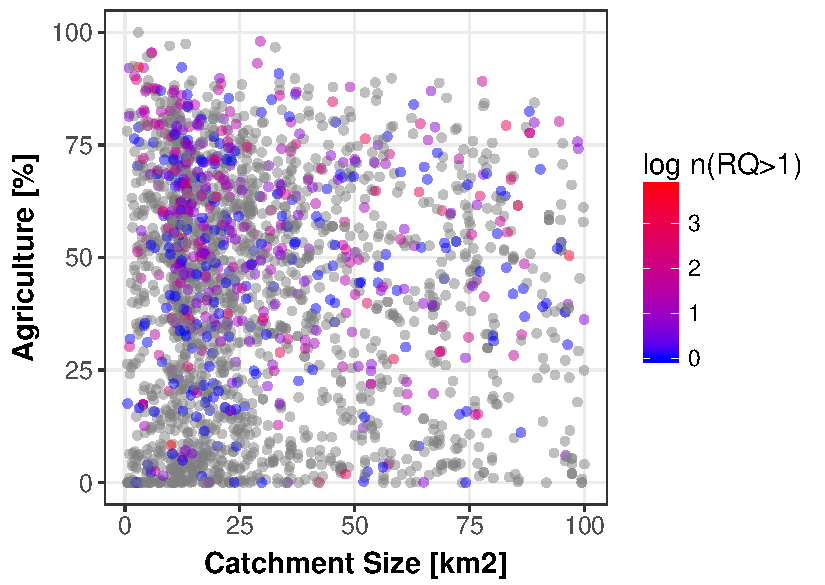
\includegraphics[width = \textwidth]{appendix/smallstreams/one/ezgagrirac}
	\caption[Raw data used for the model in equation 3.2 and Figure 3.4 of the main article.]{Raw data used for the model in equation 2 and Figure 3 of the main article. Color codes the number of RAC exceedances (on a log-scale). Grey points denote sites without any exceedance.}
	\label{fig:ezgagrirac}
\end{figure}



%% -------------------------------------------------------------------------
\clearpage
\section{Effect of precipitation and season on RQ}

\begin{figure}[H]
	\centering
	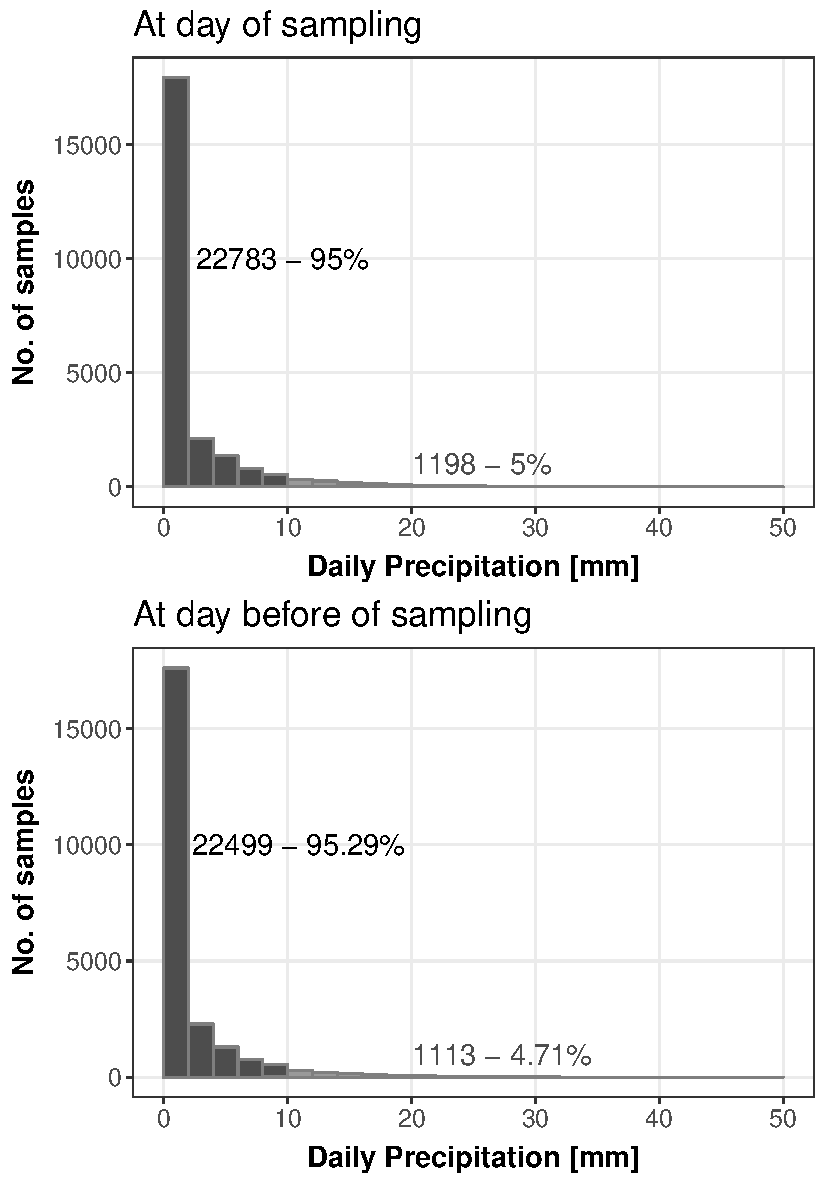
\includegraphics[width = 0.8\textwidth]{appendix/smallstreams/one/precip}
	\caption[Distribution of precipitation at sampling occasions.]{Distribution of precipitation at sampling occasions. top: at sampling date. bottom: at the day before sampling.}
	\label{fig:precip}
\end{figure}

%%% from do_precip.R
% 
\clearpage
\begin{longtable}{lp{2.5cm}rlp{1.5cm}p{1.5cm}p{1.5cm}}
\caption[23 pesticides for which we modelled the relationship with precipitation and seasonality.]{23 pesticides for which we modelled the relationship between RQ and precipitation and seasonality, respectively.
                    Order is the same as in Figure 5 of the main text. See Table \ref{tab:var_model_coef} for model coefficients.} \\ 
  \toprule
 & Name & CAS & Group & \%>LOQ & no. > LOQ & total no. \\ 
  \midrule
1 & Azoxystrobin & 131860-33-8 & fungicide & 9.58 & 644 & 6723 \\ 
  2 & Bentazon & 25057-89-0 & herbicide & 19.43 & 2313 & 11905 \\ 
  3 & Boscalid & 188425-85-6 & fungicide & 23.00 & 2175 & 9455 \\ 
  4 & Carbendazim & 10605-21-7 & fungicide & 16.10 & 582 & 3615 \\ 
  5 & Chlorpyrifos & 2921-88-2 & insecticide & 6.17 & 865 & 14026 \\ 
  6 & Clothianidin & 210880-92-5 & insecticide & 6.30 & 141 & 2237 \\ 
  7 & Diflufenican & 83164-33-4 & herbicide & 12.63 & 1867 & 14784 \\ 
  8 & Dimoxystrobin & 149961-52-4 & fungicide & 6.83 & 216 & 3164 \\ 
  9 & Diuron & 330-54-1 & herbicide & 12.07 & 2138 & 17708 \\ 
  10 & Ethofumesat & 26225-79-6 & herbicide & 5.10 & 998 & 19552 \\ 
  11 & Flufenacet & 142459-58-3 & herbicide & 5.97 & 772 & 12923 \\ 
  12 & Glyphosate & 1071-83-6 & herbicide & 40.73 & 1389 & 3410 \\ 
  13 & Imidacloprid & 138261-41-3 & insecticide & 5.88 & 176 & 2992 \\ 
  14 & Isoproturon & 34123-59-6 & herbicide & 21.84 & 3984 & 18239 \\ 
  15 & MCPA & 94-74-6 & herbicide & 12.81 & 1567 & 12237 \\ 
  16 & Mecoprop & 93-65-2 & herbicide & 12.21 & 1463 & 11984 \\ 
  17 & Metazachlor & 67129-08-2 & herbicide & 9.23 & 1930 & 20907 \\ 
  18 & Nicosulfuron & 111991-09-4 & herbicide & 5.33 & 263 & 4934 \\ 
  19 & Propiconazol & 60207-90-1 & fungicide & 5.67 & 772 & 13622 \\ 
  20 & Quinmerac & 90717-03-6 & herbicide & 13.46 & 939 & 6974 \\ 
  21 & Tebuconazol & 107534-96-3 & fungicide & 6.08 & 968 & 15924 \\ 
  22 & Terbuthylazin & 5915-41-3 & herbicide & 14.59 & 3142 & 21540 \\ 
   \bottomrule
\label{tab:var_model}
\end{longtable}

\clearpage
\begin{landscape}
\begingroup\fontsize{8pt}{10pt}\selectfont
\begin{longtable}{lp{2cm}p{0.6cm}p{1.8cm}p{1.8cm}p{1.8cm}p{1.8cm}p{1.8cm}p{1.8cm}}
\caption[Coefficients and CI from per compound models.]{Coefficients and CI from per compound models. 
                     Bold values denote coefficients where the CI for precipitation encompasses zero.
                     Coefficients are on the link scale (log for $\mu$ and logit for $\nu$).} \\ 
  \toprule
 & Compound & effect & $log~precip_0$ & $log~precip_{-1}$ & Quarter 1 & Quarter 2 & Quarter 3 & Quarter 4 \\ 
  \midrule
  \endfirsthead
  %
  \caption*{\raggedright Table \thetable\ Continued. }\\
  \toprule
 & Compound & effect & $log~precip_0$ & $log~precip_{-1}$ & Quarter 1 & Quarter 2 & Quarter 3 & Quarter 4 \\ 
  \midrule
  \endhead
%
1 & Azoxystrobin & $\mu$ & \textbf{0.23}\newline (0.15 - 0.31) & 0.04\newline (-0.03 - 0.12) & -3.39\newline (-3.56 - -3.22) & -3.02\newline (-3.14 - -2.89) & -3.16\newline (-3.29 - -3.03) & -3.47\newline (-3.63 - -3.3) \\ 
  2 & Bentazon & $\mu$ & -0.03\newline (-0.07 - 0) & 0.02\newline (-0.02 - 0.05) & -9.46\newline (-9.53 - -9.38) & -8.97\newline (-9.02 - -8.92) & -9.14\newline (-9.2 - -9.07) & -9.46\newline (-9.53 - -9.39) \\ 
  3 & Boscalid & $\mu$ & \textbf{0.06}\newline (0.02 - 0.1) & \textbf{0.1}\newline (0.06 - 0.13) & -6.72\newline (-6.79 - -6.64) & -6.42\newline (-6.49 - -6.36) & -6.51\newline (-6.58 - -6.45) & -6.58\newline (-6.65 - -6.5) \\ 
  4 & Carbendazim & $\mu$ & \textbf{-0.1}\newline (-0.16 - -0.03) & \textbf{0.16}\newline (0.09 - 0.22) & -2.42\newline (-2.58 - -2.27) & -1.95\newline (-2.05 - -1.84) & -2.11\newline (-2.22 - -2) & -2.32\newline (-2.46 - -2.18) \\ 
  5 & Chlorpyrifos & $\mu$ & \textbf{0.08}\newline (0.04 - 0.13) & -0.03\newline (-0.08 - 0.01) & 0.85\newline (0.77 - 0.93) & 1\newline (0.93 - 1.06) & 0.9\newline (0.82 - 0.98) & 0.94\newline (0.86 - 1.03) \\ 
  6 & Clothianidin & $\mu$ & 0.08\newline (-0.04 - 0.19) & -0.1\newline (-0.21 - 0.02) & 0.94\newline (0.77 - 1.12) & 0.67\newline (0.49 - 0.84) & 1.02\newline (0.8 - 1.25) & 1.55\newline (1.32 - 1.78) \\ 
  7 & Diflufenican & $\mu$ & -0.02\newline (-0.06 - 0.02) & \textbf{0.05}\newline (0.02 - 0.09) & -0.56\newline (-0.62 - -0.5) & -1.01\newline (-1.07 - -0.94) & -1.08\newline (-1.16 - -1) & -0.71\newline (-0.77 - -0.65) \\ 
  8 & Dimoxystrobin & $\mu$ & \textbf{0.35}\newline (0.2 - 0.5) & 0.02\newline (-0.15 - 0.19) & -1.17\newline (-1.44 - -0.89) & -0.42\newline (-0.64 - -0.2) & -0.07\newline (-0.39 - 0.25) & -0.02\newline (-0.35 - 0.31) \\ 
  9 & Diuron & $\mu$ & 0\newline (-0.03 - 0.03) & \textbf{0.07}\newline (0.04 - 0.1) & -2.72\newline (-2.83 - -2.61) & -2.43\newline (-2.47 - -2.39) & -2.48\newline (-2.53 - -2.44) & -2.64\newline (-2.71 - -2.58) \\ 
  10 & Ethofumesat & $\mu$ & \textbf{0.12}\newline (0.06 - 0.17) & 0.01\newline (-0.05 - 0.06) & -6.11\newline (-6.27 - -5.96) & -5.49\newline (-5.56 - -5.42) & -6.18\newline (-6.29 - -6.08) & -6.1\newline (-6.24 - -5.95) \\ 
  11 & Flufenacet & $\mu$ & 0.03\newline (-0.02 - 0.08) & \textbf{0.05}\newline (0.01 - 0.1) & -3.71\newline (-3.79 - -3.62) & -3.7\newline (-3.81 - -3.59) & -3.29\newline (-3.44 - -3.15) & -3.63\newline (-3.68 - -3.57) \\ 
  12 & Glyphosate & $\mu$ & -0.04\newline (-0.09 - 0.01) & \textbf{0.14}\newline (0.09 - 0.19) & -6.3\newline (-6.46 - -6.13) & -6.08\newline (-6.16 - -6) & -5.73\newline (-5.8 - -5.66) & -6.11\newline (-6.21 - -6.01) \\ 
  13 & Imidacloprid & $\mu$ & 0\newline (-0.08 - 0.09) & -0.01\newline (-0.09 - 0.07) & 0.61\newline (0.33 - 0.88) & 1.15\newline (1.02 - 1.27) & 1.4\newline (1.28 - 1.53) & 1.24\newline (1.06 - 1.42) \\ 
  14 & Isoproturon & $\mu$ & 0.02\newline (-0.02 - 0.05) & \textbf{0.21}\newline (0.17 - 0.24) & -3.29\newline (-3.37 - -3.22) & -3.01\newline (-3.06 - -2.96) & -3.43\newline (-3.5 - -3.35) & -2.79\newline (-2.84 - -2.73) \\ 
  15 & MCPA & $\mu$ & 0.04\newline (-0.01 - 0.09) & \textbf{0.09}\newline (0.04 - 0.14) & -5.07\newline (-5.27 - -4.87) & -4.25\newline (-4.32 - -4.19) & -4.48\newline (-4.57 - -4.4) & -4.7\newline (-4.81 - -4.58) \\ 
  16 & Mecoprop & $\mu$ & 0.04\newline (-0.01 - 0.09) & \textbf{0.05}\newline (0.01 - 0.1) & -8.36\newline (-8.49 - -8.22) & -7.59\newline (-7.65 - -7.52) & -7.77\newline (-7.85 - -7.69) & -8.07\newline (-8.18 - -7.97) \\ 
  17 & Metazachlor & $\mu$ & \textbf{-0.07}\newline (-0.12 - -0.02) & \textbf{0.09}\newline (0.04 - 0.13) & -2.97\newline (-3.06 - -2.88) & -2.94\newline (-3.04 - -2.85) & -2.21\newline (-2.28 - -2.14) & -2.77\newline (-2.84 - -2.7) \\ 
  18 & Nicosulfuron & $\mu$ & \textbf{0.23}\newline (0.12 - 0.34) & \textbf{-0.28}\newline (-0.39 - -0.18) & -0.98\newline (-1.22 - -0.74) & -0.2\newline (-0.36 - -0.03) & -0.07\newline (-0.25 - 0.11) & -0.97\newline (-1.16 - -0.78) \\ 
  19 & Propiconazol & $\mu$ & \textbf{0.08}\newline (0.02 - 0.14) & 0.01\newline (-0.05 - 0.07) & -3.99\newline (-4.15 - -3.83) & -3.63\newline (-3.71 - -3.55) & -3.82\newline (-3.91 - -3.72) & -3.63\newline (-3.74 - -3.53) \\ 
  20 & Quinmerac & $\mu$ & 0.02\newline (-0.05 - 0.09) & 0.05\newline (-0.01 - 0.12) & -9.08\newline (-9.19 - -8.96) & -9.12\newline (-9.24 - -9) & -8.46\newline (-8.59 - -8.33) & -8.64\newline (-8.72 - -8.55) \\ 
  21 & Tebuconazol & $\mu$ & -0.01\newline (-0.06 - 0.03) & \textbf{0.09}\newline (0.04 - 0.14) & -2.17\newline (-2.28 - -2.06) & -1.93\newline (-2 - -1.86) & -2.2\newline (-2.28 - -2.11) & -2.15\newline (-2.24 - -2.06) \\ 
  22 & Terbuthylazin & $\mu$ & \textbf{0.09}\newline (0.06 - 0.13) & \textbf{0.11}\newline (0.08 - 0.15) & -3.65\newline (-3.73 - -3.56) & -2.78\newline (-2.84 - -2.73) & -3.25\newline (-3.3 - -3.19) & -3.52\newline (-3.59 - -3.44) \\ 
   \midrule
23 & Azoxystrobin & $\nu$ & 0\newline (-0.13 - 0.13) & \textbf{0.24}\newline (0.11 - 0.37) & -3.5\newline (-3.76 - -3.25) & -2.33\newline (-2.54 - -2.13) & -2.14\newline (-2.36 - -1.92) & -3.2\newline (-3.45 - -2.95) \\ 
  24 & Bentazon & $\nu$ & 0\newline (-0.08 - 0.08) & 0.05\newline (-0.03 - 0.13) & -2.26\newline (-2.44 - -2.09) & -1.53\newline (-1.65 - -1.4) & -1.88\newline (-2.02 - -1.74) & -2.25\newline (-2.4 - -2.11) \\ 
  25 & Boscalid & $\nu$ & -0.01\newline (-0.1 - 0.08) & \textbf{0.45}\newline (0.37 - 0.54) & -1.99\newline (-2.16 - -1.82) & -1.22\newline (-1.36 - -1.07) & -1.24\newline (-1.38 - -1.09) & -1.81\newline (-1.96 - -1.65) \\ 
  26 & Carbendazim & $\nu$ & 0.09\newline (-0.04 - 0.22) & \textbf{0.19}\newline (0.06 - 0.32) & -2.72\newline (-3 - -2.44) & -1.49\newline (-1.69 - -1.28) & -1.26\newline (-1.48 - -1.04) & -2.31\newline (-2.56 - -2.06) \\ 
  27 & Chlorpyrifos & $\nu$ & \textbf{0.11}\newline (0.01 - 0.21) & 0.1\newline (0 - 0.19) & -3.27\newline (-3.45 - -3.1) & -2.63\newline (-2.79 - -2.48) & -3.22\newline (-3.39 - -3.05) & -3.42\newline (-3.61 - -3.23) \\ 
  28 & Clothianidin & $\nu$ & -0.05\newline (-0.3 - 0.2) & 0.19\newline (-0.07 - 0.44) & -2.66\newline (-3.06 - -2.26) & -2.58\newline (-2.97 - -2.19) & -3.19\newline (-3.69 - -2.69) & -3.93\newline (-4.46 - -3.41) \\ 
  29 & Diflufenican & $\nu$ & 0.06\newline (-0.02 - 0.14) & \textbf{0.26}\newline (0.17 - 0.34) & -1.89\newline (-2.03 - -1.75) & -2.45\newline (-2.59 - -2.31) & -3.14\newline (-3.3 - -2.98) & -2.09\newline (-2.22 - -1.95) \\ 
  30 & Dimoxystrobin & $\nu$ & 0.19\newline (-0.02 - 0.41) & \textbf{0.23}\newline (0.01 - 0.46) & -3.37\newline (-3.78 - -2.96) & -2.25\newline (-2.58 - -1.91) & -3.14\newline (-3.55 - -2.72) & -3.58\newline (-4.02 - -3.15) \\ 
  31 & Diuron & $\nu$ & 0.05\newline (-0.01 - 0.12) & \textbf{0.28}\newline (0.22 - 0.35) & -3.88\newline (-4.09 - -3.67) & -1.67\newline (-1.76 - -1.58) & -1.74\newline (-1.84 - -1.63) & -2.72\newline (-2.85 - -2.6) \\ 
  32 & Ethofumesat & $\nu$ & 0.09\newline (-0.01 - 0.18) & \textbf{0.21}\newline (0.12 - 0.3) & -4.39\newline (-4.63 - -4.16) & -2.23\newline (-2.35 - -2.11) & -3.49\newline (-3.66 - -3.32) & -4.23\newline (-4.44 - -4.01) \\ 
  33 & Flufenacet & $\nu$ & \textbf{0.16}\newline (0.06 - 0.27) & \textbf{0.59}\newline (0.49 - 0.69) & -2.57\newline (-2.75 - -2.39) & -3.8\newline (-4.01 - -3.58) & -4.17\newline (-4.44 - -3.89) & -1.76\newline (-1.88 - -1.64) \\ 
  34 & Glyphosate & $\nu$ & 0.11\newline (0 - 0.23) & \textbf{0.29}\newline (0.18 - 0.4) & -1.79\newline (-2.09 - -1.48) & -0.12\newline (-0.3 - 0.05) & 0.34\newline (0.17 - 0.51) & -0.53\newline (-0.73 - -0.32) \\ 
  35 & Imidacloprid & $\nu$ & -0.01\newline (-0.26 - 0.25) & -0.1\newline (-0.34 - 0.15) & -4.68\newline (-5.35 - -4) & -3.04\newline (-3.41 - -2.68) & -2.83\newline (-3.21 - -2.45) & -4.07\newline (-4.56 - -3.58) \\ 
  36 & Isoproturon & $\nu$ & 0.04\newline (-0.02 - 0.09) & \textbf{0.31}\newline (0.25 - 0.36) & -1.82\newline (-1.93 - -1.7) & -1.19\newline (-1.27 - -1.12) & -2.11\newline (-2.22 - -2.01) & -0.8\newline (-0.88 - -0.72) \\ 
  37 & MCPA & $\nu$ & -0.06\newline (-0.13 - 0.02) & \textbf{0.35}\newline (0.28 - 0.42) & -3.79\newline (-4.04 - -3.54) & -1.27\newline (-1.37 - -1.18) & -1.81\newline (-1.93 - -1.68) & -2.77\newline (-2.92 - -2.62) \\ 
  38 & Mecoprop & $\nu$ & 0.07\newline (-0.01 - 0.15) & \textbf{0.35}\newline (0.27 - 0.42) & -3.04\newline (-3.23 - -2.84) & -1.56\newline (-1.67 - -1.45) & -1.89\newline (-2.02 - -1.76) & -2.71\newline (-2.86 - -2.56) \\ 
  39 & Metazachlor & $\nu$ & 0.06\newline (-0.01 - 0.13) & \textbf{0.21}\newline (0.14 - 0.27) & -2.81\newline (-2.94 - -2.67) & -3.22\newline (-3.36 - -3.09) & -2.11\newline (-2.22 - -2.01) & -2.05\newline (-2.16 - -1.95) \\ 
  40 & Nicosulfuron & $\nu$ & \textbf{0.2}\newline (0.01 - 0.39) & \textbf{0.26}\newline (0.07 - 0.45) & -3.87\newline (-4.27 - -3.48) & -2.96\newline (-3.26 - -2.66) & -2.99\newline (-3.3 - -2.68) & -3.23\newline (-3.56 - -2.9) \\ 
  41 & Propiconazol & $\nu$ & -0.02\newline (-0.13 - 0.09) & \textbf{0.39}\newline (0.29 - 0.5) & -4.05\newline (-4.32 - -3.78) & -2.72\newline (-2.88 - -2.57) & -2.88\newline (-3.06 - -2.7) & -3.43\newline (-3.63 - -3.24) \\ 
  42 & Quinmerac & $\nu$ & -0.03\newline (-0.13 - 0.08) & \textbf{0.32}\newline (0.22 - 0.42) & -2.23\newline (-2.43 - -2.02) & -2.58\newline (-2.76 - -2.41) & -2.49\newline (-2.69 - -2.29) & -1.2\newline (-1.34 - -1.06) \\ 
  43 & Tebuconazol & $\nu$ & \textbf{0.1}\newline (0.01 - 0.2) & \textbf{0.3}\newline (0.21 - 0.39) & -3.41\newline (-3.61 - -3.2) & -2.66\newline (-2.8 - -2.53) & -2.9\newline (-3.06 - -2.75) & -3.17\newline (-3.34 - -3) \\ 
  44 & Terbuthylazin & $\nu$ & \textbf{0.06}\newline (0.01 - 0.12) & \textbf{0.28}\newline (0.22 - 0.33) & -2.92\newline (-3.05 - -2.79) & -1.45\newline (-1.53 - -1.37) & -1.48\newline (-1.57 - -1.39) & -2.47\newline (-2.58 - -2.37) \\ 
   \bottomrule
\label{tab:var_model_coef}
\end{longtable}
\endgroup
\end{landscape}


\begin{figure}
	\centering
	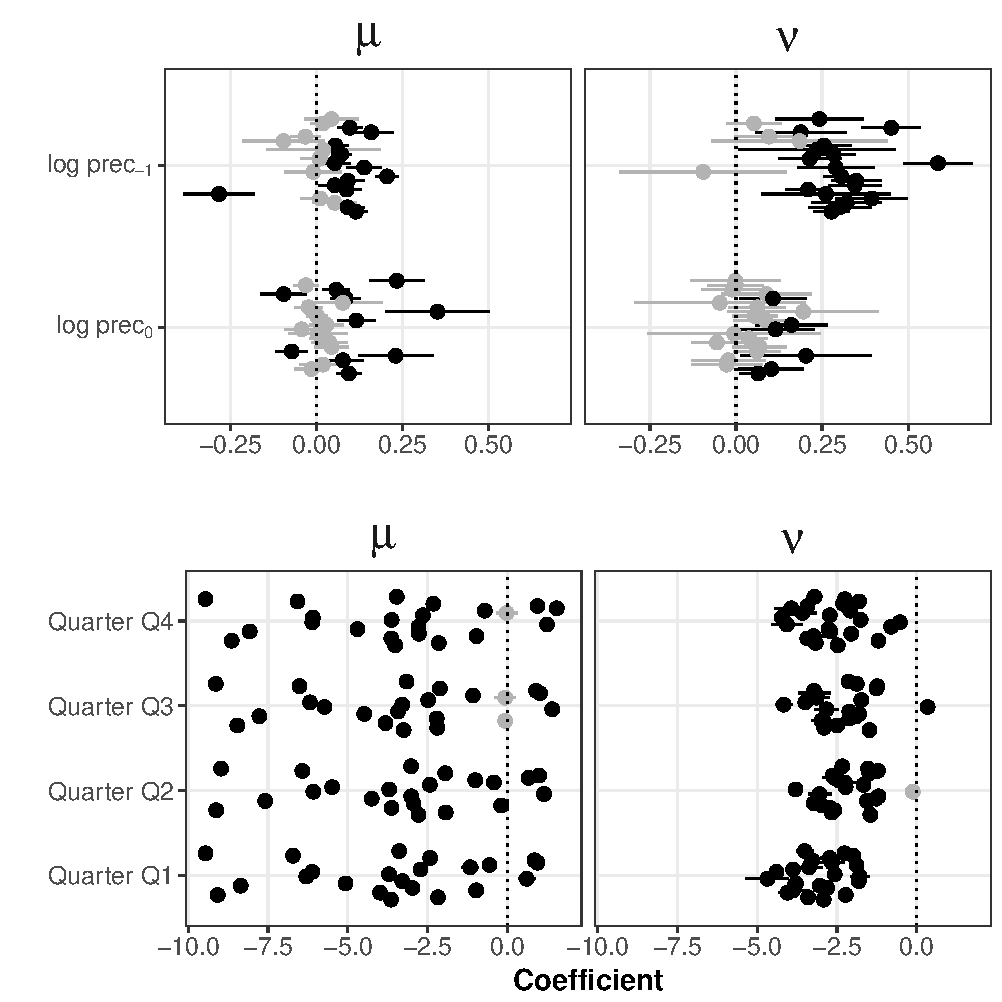
\includegraphics[width = 0.95\textwidth]{appendix/smallstreams/one/coefs}
	\caption[Graphical representation of coefficients from table \ref{tab:var_model_coef}.]{Graphical representation of coefficients from table \ref{tab:var_model_coef}. Top row: Effect of precipitation at the day before sampling and at day of sampling. Bottom row: estimates for the four Quarters. Each dot represents one compound (in the order described in table \ref{tab:var_model}). Coefficients where the CI encompasses zero are shown in gray colour. Coefficients are shown on the link scale (log for $\mu$ and logit for $\nu$).}
	\label{fig:coefs}
\end{figure}
% 


%% -------------------------------------------------------------------------
\clearpage
\section{Pesticides in small streams}
%% from do_pollution.R
\vspace{-0.5cm}
\begin{longtable}{p{2.5cm}rR{1cm}R{1cm}R{1.2cm}R{1.2cm}R{1.3cm}}
\caption[Overview on RAC exceedances of the 78 compounds with more than 1000 measurements.]{Overview on RAC exceedances of the 78 compounds with more than 1000 measurements. No. = number of measurements;  \% RQ \textgreater 1 = RAC exceedances; \% RQ \textgreater 1 | \textgreater LOQ= RAC exceedances as fraction of detects.} \\ 
  \toprule
Name & No.  & No. \textgreater LOQ & \% \textgreater LOQ & No. RQ \textgreater 1 & \% RQ \textgreater 1 & \% RQ \textgreater 1 | \textgreater LOQ \\ 
  \midrule
  \endfirsthead
  %
\caption*{\raggedright Table \thetable\ Continued. }\\
\toprule
Name & No.  & No. \textgreater LOQ & \% \textgreater LOQ & No. RQ \textgreater 1 & \% RQ \textgreater 1 & \% RQ \textgreater 1 | \textgreater LOQ \\ 
\midrule
\endhead
%
2,4-D & 12290 & 284 & 2.3 & 10 & 0.1 & 3.5 \\ 
  Aclonifen & 9861 & 67 & 0.7 &  4 & 0.0 & 6.0 \\ 
  Azoxystrobin & 7059 & 690 & 9.8 &  6 & 0.1 & 0.9 \\ 
  Benalaxyl & 6964 & 10 & 0.1 &  0 & 0.0 & 0.0 \\ 
  Bentazon & 12429 & 2421 & 19.5 &  0 & 0.0 & 0.0 \\ 
  Bifenthrin & 1353 &  0 & 0.0 &  0 & 0.0 &  \\ 
  Boscalid & 9886 & 2296 & 23.2 &  0 & 0.0 & 0.0 \\ 
  Bromoxynil & 9451 & 78 & 0.8 &  0 & 0.0 & 0.0 \\ 
  Carbendazim & 3851 & 654 & 17.0 & 12 & 0.3 & 1.8 \\ 
  Chloridazon & 15724 & 511 & 3.2 &  0 & 0.0 & 0.0 \\ 
  Chlorpyrifos & 14704 & 954 & 6.5 & 838 & 5.7 & 87.8 \\ 
  Chlortoluron & 18286 & 371 & 2.0 &  2 & 0.0 & 0.5 \\ 
  Clomazon & 9268 & 440 & 4.7 &  0 & 0.0 & 0.0 \\ 
  Clopyralid & 5520 & 107 & 1.9 &  0 & 0.0 & 0.0 \\ 
  Clothianidin & 2409 & 154 & 6.4 & 123 & 5.1 & 79.9 \\ 
  Cypermetryn & 1428 &  5 & 0.4 &  1 & 0.1 & 20.0 \\ 
  Cyprodinil & 9779 & 118 & 1.2 &  0 & 0.0 & 0.0 \\ 
  Dicamba & 7641 & 76 & 1.0 &  0 & 0.0 & 0.0 \\ 
  Difenoconazol & 1644 & 11 & 0.7 &  2 & 0.1 & 18.2 \\ 
  Diflufenican & 15457 & 1932 & 12.5 & 273 & 1.8 & 14.1 \\ 
  Dimefuron & 7833 &  5 & 0.1 &  0 & 0.0 & 0.0 \\ 
  Dimethachlor & 8858 & 344 & 3.9 &  0 & 0.0 & 0.0 \\ 
  Dimethoat & 14423 & 185 & 1.3 &  1 & 0.0 & 0.5 \\ 
  Dimethomorph & 2316 & 91 & 3.9 &  0 & 0.0 & 0.0 \\ 
  Dimoxystrobin & 3370 & 232 & 6.9 & 49 & 1.5 & 21.1 \\ 
  Diuron & 18560 & 2336 & 12.6 & 40 & 0.2 & 1.7 \\ 
  Epoxiconazol & 16454 & 621 & 3.8 &  7 & 0.0 & 1.1 \\ 
  Ethofumesat & 20430 & 1078 & 5.3 &  0 & 0.0 & 0.0 \\ 
  Fenhexamid & 2690 & 42 & 1.6 &  0 & 0.0 & 0.0 \\ 
  Fenpropimorph & 12850 & 199 & 1.5 &  5 & 0.0 & 2.5 \\ 
  Fluazifop & 3022 & 57 & 1.9 &  0 & 0.0 & 0.0 \\ 
  Fluazifop-P & 4033 & 14 & 0.3 &  0 & 0.0 & 0.0 \\ 
  Fluazifop-P-butyl & 1728 &  0 & 0.0 &  0 & 0.0 &  \\ 
  Fluazifop-butyl & 1287 &  0 & 0.0 &  0 & 0.0 &  \\ 
  Fludioxonil & 3203 & 42 & 1.3 &  1 & 0.0 & 2.4 \\ 
  Flufenacet & 13509 & 798 & 5.9 &  1 & 0.0 & 0.1 \\ 
  Fluquinconazole & 6762 & 117 & 1.7 &  0 & 0.0 & 0.0 \\ 
  Fluroxypyr & 8096 & 378 & 4.7 &  0 & 0.0 & 0.0 \\ 
  Flurtamone & 16958 & 638 & 3.8 &  2 & 0.0 & 0.3 \\ 
  Flusilazol & 5257 & 53 & 1.0 &  1 & 0.0 & 1.9 \\ 
  Glyphosate & 3557 & 1455 & 40.9 &  1 & 0.0 & 0.1 \\ 
  Imidacloprid & 3169 & 192 & 6.1 & 169 & 5.3 & 88.0 \\ 
  Ioxynil & 8114 & 20 & 0.2 &  0 & 0.0 & 0.0 \\ 
  Isoproturon & 19112 & 4164 & 21.8 & 92 & 0.5 & 2.2 \\ 
  Kresoxim-methyl & 6929 & 14 & 0.2 &  0 & 0.0 & 0.0 \\ 
  Lenacil & 13837 & 183 & 1.3 &  0 & 0.0 & 0.0 \\ 
  MCPA & 12773 & 1687 & 13.2 &  2 & 0.0 & 0.1 \\ 
  Mecoprop & 12521 & 1552 & 12.4 &  0 & 0.0 & 0.0 \\ 
  Metalaxyl & 14460 & 299 & 2.1 &  0 & 0.0 & 0.0 \\ 
  Metamitron & 15390 & 613 & 4.0 &  0 & 0.0 & 0.0 \\ 
  Metazachlor & 21906 & 2015 & 9.2 & 55 & 0.3 & 2.7 \\ 
  Methamidophos & 1303 &  0 & 0.0 &  0 & 0.0 &  \\ 
  Methobromuron & 14968 & 24 & 0.2 &  1 & 0.0 & 4.2 \\ 
  Metribuzin & 15411 & 192 & 1.2 & 15 & 0.1 & 7.8 \\ 
  Napropamid & 9914 & 269 & 2.7 &  1 & 0.0 & 0.4 \\ 
  Nicosulfuron & 5172 & 288 & 5.6 & 77 & 1.5 & 26.7 \\ 
  Penconazol & 4846 & 159 & 3.3 &  0 & 0.0 & 0.0 \\ 
  Pendimethalin & 16997 & 328 & 1.9 &  4 & 0.0 & 1.2 \\ 
  Pethoxamid & 3102 & 37 & 1.2 &  0 & 0.0 & 0.0 \\ 
  Phoxim & 1492 &  0 & 0.0 &  0 & 0.0 &  \\ 
  Picolinafen & 8901 & 11 & 0.1 &  2 & 0.0 & 18.2 \\ 
  Picoxystrobin & 3620 &  7 & 0.2 &  0 & 0.0 & 0.0 \\ 
  Pirimicarb & 11330 & 232 & 2.0 & 27 & 0.2 & 11.6 \\ 
  Prochloraz & 5795 & 33 & 0.6 &  0 & 0.0 & 0.0 \\ 
  Propiconazol & 14250 & 818 & 5.7 &  7 & 0.0 & 0.9 \\ 
  Propyzamid & 11937 & 453 & 3.8 &  0 & 0.0 & 0.0 \\ 
  Prosulfocarb & 5001 & 126 & 2.5 &  0 & 0.0 & 0.0 \\ 
  Pyrimethanil & 8136 & 122 & 1.5 &  0 & 0.0 & 0.0 \\ 
  Quinmerac & 7291 & 989 & 13.6 &  0 & 0.0 & 0.0 \\ 
  Rimsulfuron & 1240 &  2 & 0.2 &  0 & 0.0 & 0.0 \\ 
  Spiroxamin & 2469 & 109 & 4.4 &  1 & 0.0 & 0.9 \\ 
  Tebuconazol & 16584 & 1024 & 6.2 & 26 & 0.2 & 2.5 \\ 
  Terbuthylazin & 22568 & 3370 & 14.9 & 35 & 0.2 & 1.0 \\ 
  Thiacloprid & 3540 & 85 & 2.4 & 85 & 2.4 & 100.0 \\ 
  Thiamethoxam & 1853 & 39 & 2.1 &  7 & 0.4 & 17.9 \\ 
  Triadimenol & 3067 & 51 & 1.7 &  0 & 0.0 & 0.0 \\ 
  Triazophos & 3588 &  2 & 0.1 &  1 & 0.0 & 50.0 \\ 
  Trifloxystrobin & 3674 & 10 & 0.3 &  1 & 0.0 & 10.0 \\
   \bottomrule
\label{tab:rac_dat}
\end{longtable}


\begin{figure}[ht]
	\centering
	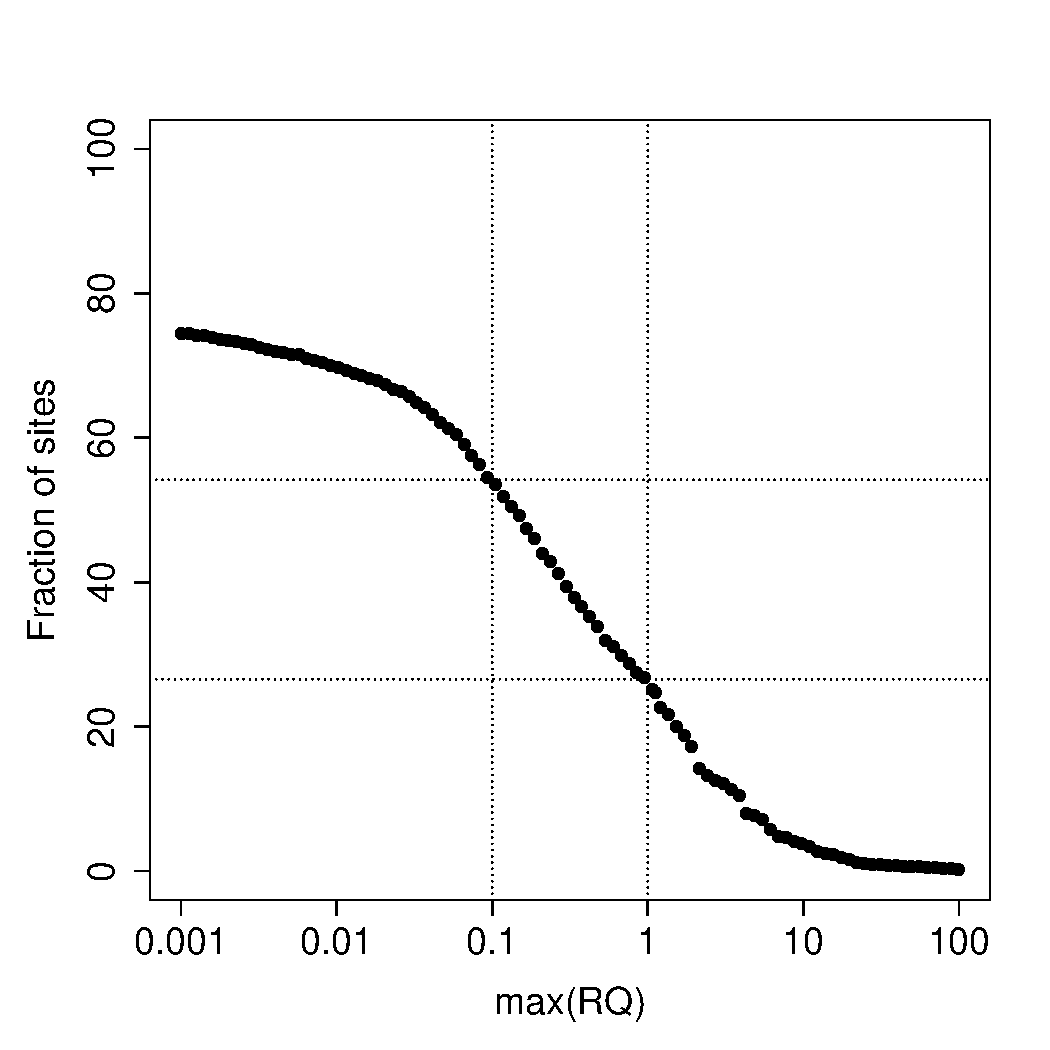
\includegraphics[width = 0.8\textwidth]{appendix/smallstreams/one/prac_ex}
	\caption[Cumulative distribution of the number sites exceeding RAC.]{Cumulative distribution of sites exceeding RAC. Dotted lines indicate fraction of sites exceeding a RQ of 1 and 0.1. 23\% of the sites showed no detection of compounds with available RAC values and are not shown due to logarithmic x-axis.}
	\label{fig:prac_ex}
\end{figure}


\begin{landscape}
\begin{figure}[ht]
	\centering
	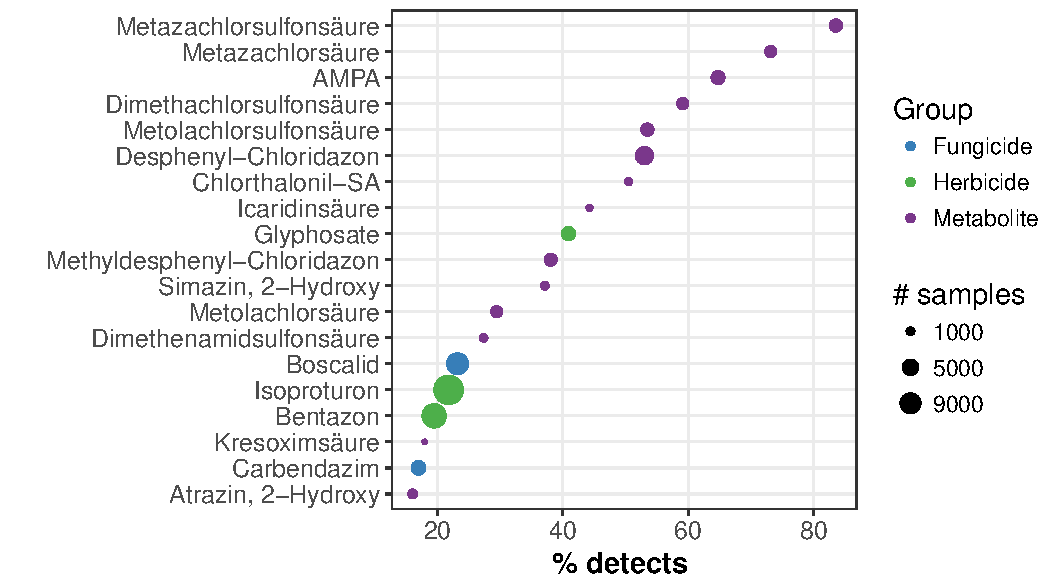
\includegraphics[width = 0.8\textheight]{appendix/smallstreams/one/pdetects}
	\caption[Proportion of samples with detects in small streams.]{Proportion of samples with detects in small streams. Only Compounds with more than 100 samples and 15\% of detects are shown.}
	\label{fig:pdetects}
\end{figure}
\end{landscape}

\begin{figure}[ht]
	\centering
	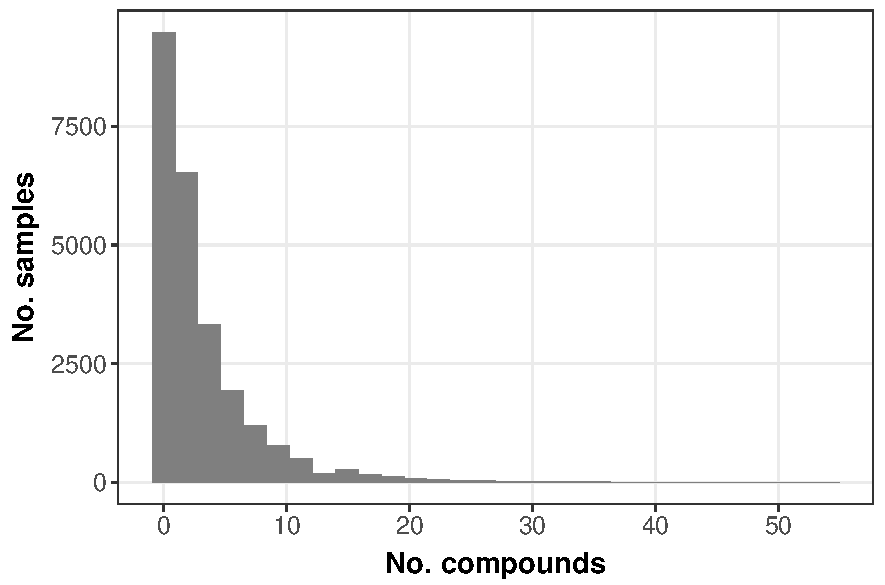
\includegraphics[width = 0.9\textwidth]{appendix/smallstreams/one/pmix}
	\caption{Distribution of the number of quantified compounds in the samples.}
	\label{fig:pmix}
\end{figure}


\clearpage
\section{Catchment size - stream width relationship}
We studied the relationship between catchment size based on three datasets containing this informations:
Data delivered by the federal state Thuringia, \citet{vos_organic_2015} and \citet{fernandez_effects_2015} (both from Rhineland-Palatinate).
We fitted to each dataset separately and to the combined dataset a power-function.
The resulting models are shown in Figure \ref{fig:size_width}. 

\begin{figure}[ht]
	\centering
	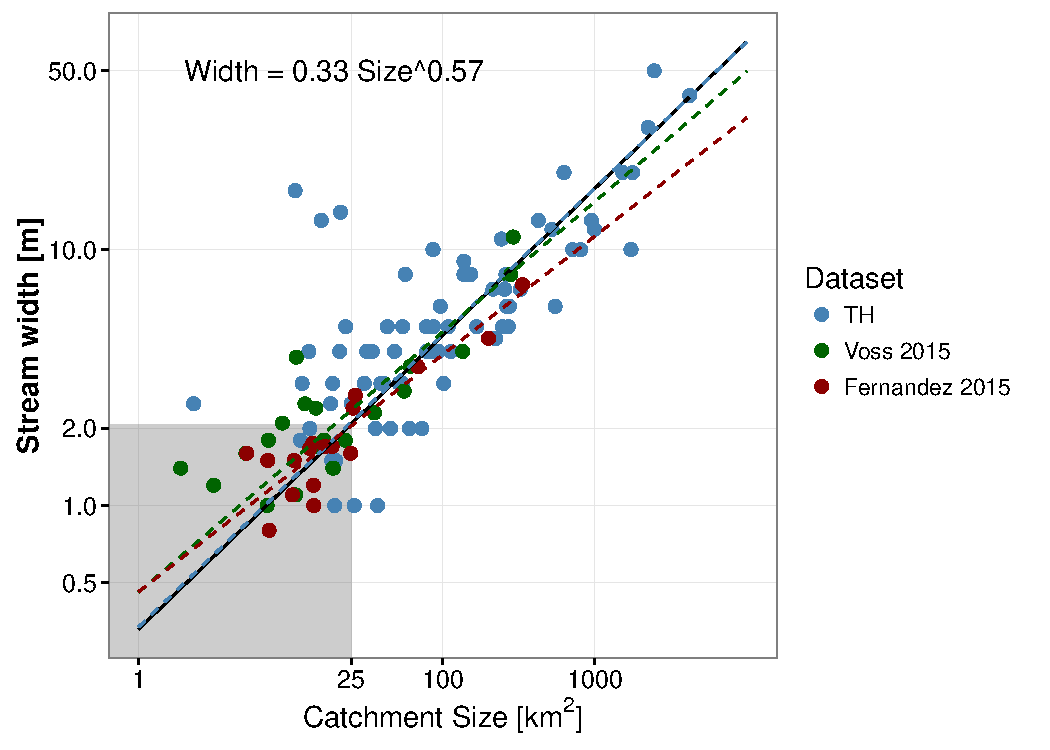
\includegraphics[width = 0.9\textwidth]{appendix/smallstreams/one/width_size}
		\caption[Relationship between catchment size and stream width.]{Relationship between catchment size and stream width. A power function has been fitted to each dataset separately (colored dashed lines) and the combined dataset (black line and equation). The gray rectangle marks the estimated catchment size for a width of 1~m (=7~km\textsuperscript{2}). }
	\label{fig:size_width}
\end{figure}

\clearpage
\section{References}
\printbibliography[heading=none]
